%\documentclass[%
%,aps%
% ,onecolumn%
%,amssymb, amsmath,
%nobibnotes, aps, prd, preprint]{revtex4-1}

\documentclass{DOEproposal}
\usepackage{amsmath, amsthm, amssymb}
\usepackage{latexsym}
\usepackage{epsfig}
\usepackage{epstopdf}
\usepackage{graphicx}
\usepackage[footnotesize,bf]{caption}
\usepackage[final]{pdfpages}
\usepackage{hyperref}
\hypersetup{
    colorlinks=true,        % false: boxed links; true: colored links
    linkcolor=blue,         % color of internal links
    citecolor=black,        % color of links to bibliography
    filecolor=magenta,      % color of file links
    urlcolor=magenta,       % color of external links
    pdfstartview=           % omit this key from pdf dictionary so reader 
}                           %     just uses user default

\usepackage{tikz}
\usetikzlibrary{shapes,arrows}
\usepackage{floatrow}
\usepackage{mathtools}
% ----------------------------------
% Things to remove!
% ----------------------------------
% Add line numbers to draft
%\usepackage{lineno}
%\linenumbers
% Lorem ipsum generator for template
%\usepackage{lipsum}
\newcommand{\lipsum}[1][1]{}
\newcommand{\TODO}{\color{red} \bf}
% Some definition to make collab. 
% editing easier. 
% ================================================
% Assign each person a color for in=text comments.
% ================================================
\usepackage[dvipsnames]{xcolor}
% For a list of named colors, see:
%     https://en.wikibooks.org/wiki/LaTeX/Colors#The_68_standard_colors_known_to_dvips

% --------------------------------------------------------------------------
% These definitions define a \NAME command which, when used like:
%    \NAME{Some comment.}
% will produce:
%    NAME says:  Some commnet.
% in the generated PDF. The comment will also be colored with NAME's color. 
% --------------------------------------------------------------------------
% A cool person 
\newcommand{\cool}[1]{{\color{Red}Cool says:~#1}}


% ----------------------------------


\newcommand{\myref}{Ref.~}
\newcommand{\myrefs}{Refs.~}
\def\wt#1{\widetilde{#1}}
\def\gsim{ \,\, \vcenter{\hbox{$\buildrel{\displaystyle >}\over\sim$}}
 \,\,}
\def\lsim{ \,\, \vcenter{\hbox{$\buildrel{\displaystyle <}\over\sim$}}
 \,\,}
\newcommand{\as}{\alpha_s}



\def\be{\begin{equation}}
\def\ee{\end{equation}}
\def\bea{\begin{eqnarray}}
\def\eea{\end{eqnarray}}

\def\beq{\begin{equation}}
\def\eeq{\end{equation}}

\newcommand{\nn}{\notag \\}

\newcommand{\CGCket}{|{\rm CGC}\rangle}
\newcommand{\CGCbra}{\langle {\rm CGC}|}


\def\vp#1{\vec{#1}_\perp}
\def\d{\dagger}
\def\lrd{\overset{\leftrightarrow}{\partial_0}}

\newcommand{\pvec}[1]{\vec{#1}\mkern2mu\vphantom{#1}}
\def\pvp#1{\pvec{#1}'_\perp}







% Use roman numerals to number all pages before the narrative.
\pagenumbering{roman}

% The PI's information
\investigator{Vladimir Skokov}
\institute{North Carolina State University}
\phone{\dots}
\email{vskokov@ncsu.edu}

% setup the title page.
% NOTE: you'll have to edit the imported file.
\title{Quantum Chromodynamics at extreme gluon densities}
\date{August 22, 2018}
\renewcommand*{\maketitle}{\begin{titlepage}
    \begin{center}
        { \Large \bf \Title }
        
        \vspace{1em}
        A proposal submitted to the DOE Office of Science \\
        \Date \\
        
        \vspace{1em}
        \emph{Funding Opportunity Announcement Number:} DE FOA 0001820 \\                                                                          
        \emph{DOE Office of Science Program Manager:} George Fai \\
        
        \vspace{1em}
        \begin{table}[h!]                                                                                         
            \centering
            \begin{tabular}{ l l }                                                                                   
                \emph{Proposing Organization:}  &  \Institute \\[1em]
                
                \emph{Principal Investigator:}  & \Investigator \\         
                & Physics Department, College of Sciences \\ 
				&North Carolina State University \\
                & Raleigh, NC 27695\\ 
                & Phone: \Phone \\ 
                & Email: \Email \\[1em]

                \emph{Requested Funding:} & {\$100/year for three years} \\
                \emph{Total Request:}     & {\$300}   \\
            \end{tabular}
        \end{table}
    
        \vspace{1em}
        Budget Summary: \\
        \vspace{0.5em}
        \begin{tabular}{|r|r|r|}                                                                                   
            \hline
            {\bf }  {\bf Year 1} & {\bf Year 2} & {\bf Year 3} \\
            \hline
             \$100K & \$100K & \$100K \\ \hline
        \end{tabular}
    \end{center}
\end{titlepage}                                                                                                         

}



\usepackage[TS1,T1]{fontenc}
\usepackage{fourier, heuristica}
\usepackage{array,longtable}
\DeclareCaptionFont{blue}{\color{LightSteelBlue3}}

\newcommand{\foo}{\color{LightSteelBlue3}\makebox[0pt]{\textbullet}\hskip-0.5pt\vrule width 1pt\hspace{\labelsep}}





%\bibliographystyle{abbrvnat}
\bibliographystyle{apsrev4-1}
\renewcommand{\v}[1]{ \ensuremath{  \vec {#1}_\perp }}
\renewcommand{\vp}[1]{ \ensuremath{  \underline {#1} }}

%%%%%%%%%%%%%%%%%%%%%%%%%%%%%%%%%%%%%%%%%%%%%%%%%%%%%%%%%%%%%%%%%%%%%%%%%%%%%%%
% Begin the document
%%%%%%%%%%%%%%%%%%%%%%%%%%%%%%%%%%%%%%%%%%%%%%%%%%%%%%%%%%%%%%%%%%%%%%%%%%%%%%%


\setlength{\textfloatsep}{10pt plus 1.0pt minus 2.0pt}
\renewcommand{\refname}{}
\begin{document}
    % make the title page
    \maketitle

    % make the table of contents
    \renewcommand{\contentsname}{Table of Contents}
    \tableofcontents
    \newpage

	\pagenumbering{arabic}
    \setcounter{page}{1}
    % the abstract
    %\phantomsection
    \section{Introduction}
    %\addcontentsline{toc}{section}{Introduction}
    %\begin{document}
\vspace{0.5em}
\noindent
{\bf Title:} \Title

\vspace{0.5em}
\noindent
{\bf Lead Institution:} \Institute

\vspace{0.5em}
\noindent
{\bf Principal Investigator:} \Investigator


\vspace{0.5em}
\noindent


\vspace{0.5em}
\noindent
{\bf Abstract:} 
Scattering processes and soft/semihard particle production in high-energy
hadron-hadron and lepton-hadron collisions are largely defined  by the 
small Bjorken $x$ component of the hadron(s) wave-function. 
These  collisions provide access to kinematic regions 
in the nucleon and nuclei where parton densities are extremely high 
and dominated by gluons. In contrast to 
well-understood dilute QCD dynamics at small distance scales, 
high gluon density QCD is an intrinsically new, nonlinear regime
forbidding usual perturbative treatment. Nevertheless due to formation of a semi-hard scale, 
the so-called saturation momentum, the theory is computable semi-analytically using 
weak coupling, but non-perturbative techniques.
This proposal aims to develope  a unifying quantitative framework for 
describing  novel aspects of small-$x$ physics in hadron-hadron,
lepton-hadron, and Ultra Peripheral A-A collisions.

This work is especially relevant to experiments at the Relativistic Heavy Ion Collider (BNL),
Large Hadron Collider (CERN) and a future Electron-Ion Collider (BNL and JLab).  


%{\TODO (should be shortened -- currently 119, the rule: 100 words or less )
%}
% participating in a collision.
%can still
%be utilized to extract   semi-analytic results for most of the observables. 


\vspace{0.5em}
\noindent
{\bf Summary of Proposed Work:}
The main objectives  are 
\begin{itemize}

	%\item Derive complete analytic results for first-saturation correction 
	%	in projectile gluon density for single inclusive and double inclusive 
	%	gluon production in classical approximation for 
	%	asymmetric collisions (e.g. proton-nucleus collisions).    

	%	Most of the semi-analytic calculations for particle production in
	%	the saturation framework are 
	%	either obtained in the dilute-dilute approximation 
	%	(fully neglecting multiple rescattering) or in dilute-dense approximation
	%	(multiple rescattering if fully accounted for in the dense target).

	%	However, to perform a systematical analysis of particle production 
	%	and correlations in hadronic collisions 
	%	it is crucial to compute the first non-trivial correction to 
	%	the dilute-dense limit. This correction is termed the first saturation correction. 

	\item Build a unified framework for a systematic 
		first-principle description of multiparticle production and
		multiparticle correlations at small $x$ in 
		various colliding systems (p-p/A and e-p/A). The critical steps include:
		\begin{itemize}
			\item Deriving complete analytic results for the first-saturation correction 
		in projectile gluon density for single inclusive and double inclusive 
		gluon production in the classical approximation for 
		asymmetric collisions (e.g. proton-nucleus collisions).
			\item Theoretical  development of a reweighting technique
		enabling an access to the high multiplicity tail of 
		hadronic wave-function/particle production. 
			\item Proper account for the small $x$ evolution in order to restore the
		three-dimensional snapshot of multi particle production in collisions
		and to elicit the dependence on the collision energy.
			\item Making the source code(s) performing numerical lattice 
				simulations for multi-particle production publicly available. 
		\end{itemize}

		{\it Potential Impact:} 
		These first-principle quantitative studies of the initial state effects in hadronic collisions 
		may lead to a potential shift of paradigm in our understanding of 
		particle production and, specificly,  the origin of collectivity. Additionally, 
		on this stage of 
		the EIC R\&D program, quantitative  predictions for the observables sensitive to 
		gluon saturation or to various gluon distribution functions  
		(e.g. the linearly polarized gluon distribution in an unpolirized hadron)  
		in the relevant energy range 
		may influence yet flexible design for EIC detectors by providing a
		optimal kinematic range for performing corresponding measurements.  

	\item Quantitatively study momentum entanglement in hadronic wave function. Derive 
		small $x$ evolution for the full density matrix including the off-diagonal components 
		in the basis of valence charge density. 
		Extract the evolution of the associated entanglement entropy. Identify potential 
		experimental observables. 

		{\it Potential impact:} Quantum entangelement is a universal phenomenon underlying 
		the behavior of quantum systems of diverse nature. The concept
		does not rely on small coupling methods and thus may facilitate extension of 
		evolution equations for entangelement entropy to an arbitrary value if the strong coupling.     
		

	\item Provide a cohesive picture of the role of quantum statistics at small $x$. 
		Study associated effects in gluon and quark production. Compute the initial state
		background contribution to the Chiral Magnetic Effect (CME). 
		
		{\it Potential impact:} Experimental data collected by CMS collaboration in p-A colisions
		challenges the conventional picture of the flow-driven CME background established in A-A
		collisions. The initial state correlations may explain the observed descrepancy.     


\end{itemize}

\vspace{0.5em}
\noindent
{\bf List of Personal:}
\begin{enumerate}
	\item Faculty: Vladimir Skokov (PI)
	\item Postdoctoral Fellows: to be hired 
	\item Graduate students:  Haowu Duan,  Gregory Johson 
\end{enumerate}


    \newpage

    % setup the main body of the proposal

    \phantomsection
    \addcontentsline{toc}{section}{Proposal Narrative}

    
    % the main body of the proposal
    \noindent

% Section 1
\section{Narrative Introduction}
    \label{sec:introduction}
    %\lipsum[5]

The 2015 Nuclear Science Advisory Committee (NSAC) Long Range Plan
\href{https://science.energy.gov/np/nsac/}
{``Reaching  for the Horizon''} outlined the key fundamental  questions{\it 
\begin{itemize}
	\item [] How are the sea quarks and gluons, and their spins, distributed in
		space and momentum inside the nucleon? 
	\item [ ] How does the nuclear environment affect the distribution of
		quarks and gluons and their interactions in nuclei?
	\item [] Where does the saturation of gluon densities set in?
\end{itemize}}
\noindent 
under one overarching theme \\
\indent {\it  
``How does subatomic matter organize itself and what phenomena emerge?''.  
} \\ \noindent 
The scientific  urge to answer these questions lead the NSAC 
to recommend EIC as the ``highest priority for new facility construction
following the completion of FRIB''. In the mid 2018, this recommendation 
was supported by the National Academy of Science which  concluded 
``that the science questions
regarding the building blocks of matter are compelling and that an EIC is
essential to answering these questions.'' 
This, however, can only be achieved   
with appropriate theoretical support %in the form of providing prediction 
and development of new theoretical tools built upon 
first-princliple approaches  to 
the theory of strong interactions. 
This proposal seeks funding for building such a tool 
with a broader application range which includes also high energy hadron-hadron 
collisions and Ultra Peripheral Collisions (UPC) of proton-nucleus and nucleus-nucleus.   

Besides the EIC physics, 
the successful implementation of the proposal will have a significant impact on 
understanding the results of other planned or on-going experimental programs  at the large 
facilities in the U.S. (RHIC, CEBAF) and Europe (CERN). 





    \vspace{0.5em}
    \subsection{Motivation}
        \label{sec:motivation}
        The two decades worth of experimental
measurements at RHIC and, then, the LHC 
have provided many unexpected results, including 
strong evidence for the formation of 
a strongly coupled plasma of quarks and gluons in
heavy-ion collisions at high energy~\cite{Shuryak:2003xe,Shuryak:2004cy,Adams:2005dq,Song:2010mg}. 
This plasma  
demonstrated properties of a nearly perfect fluid; 
this fact facilitated a  theoretical description 
of the collisions dynamics
in the framework of hydrodynamics starting just  
about 1 fm/c after the heavy-ion impact~\cite{Schafer:2009dj,Song:2010mg,Romatschke:2017ejr}.   

The success of the hydrodynamic description, however, cannot be complete 
without a detailed understanding of the initial 
non-equilibrium state. The properties of this state go beyond the range of applicability 
of hydrodynamics and  are little known; 
the evolution of this state towards equilibrated 
thermal nearly perfect liquid  is not well understood. 
One dominant mechanism describing the initial phase is 
based on the saturation framework, also widely known as 
the Color Glass Condensate~\cite{Iancu:2002xk,Albacete:2014fwa,KovchegovLevin}. According to the framework, the 
high energy particle production and scattering processes are 
dominated by the classical gluon fields providing a 
background for systematic weak-coupling 
computation of quantum correction on top of it.  

Under laboratory conditions, 
collisions of heavy-ions create probably the most optimal envi\-ronment for 
probing quark-gluon plasma near equilibrium, but 
at the same time they are poorly suited to study the 
initial state particle production. This is because 
most of the observables in heavy-ion collisions are 
sensitive not only to  initial state, but also 
to  final sate interactions. However, to uniquely map the transport properties 
of the plasma, it is critical to extract information 
about the initial state in collisions where 
the final state is better understood and the 
initial state is expected to play the dominant role.
This necessitates probing a nucleus  and a nucleon with the smallest projectiles: 
proton and ultimately electron. 
Theoretically, a controlled,  first principle description of such collisions (p-p, p-A, e-A) 
is not as complex as A-A collisions 
and at high energy can be performed in a common quantitative framework: the saturation framework. 
Later on, the results of the framework may be transferred to describe the initial state of A-A collisions. 


One example of a similar strategy was realized recently in Refs.~\cite{Mantysaari:2016ykx,Mantysaari:2016jaz,Mantysaari:2017cni} 
where the saturation motivated model (IP-SAT, see Ref.~\cite{Kowalski:2003hm}) for e-p collisions  was used to constrain the 
shape fluctuations of the proton wave function by studying 
coherent and incoherent diffractive 
vector meson production at HERA. The proton shape fluctuations may have a direct 
impact on properties of the matter created in A-A collisions from 
the initial state in peripheral to ultra central collisions. 



Theoretical analysis of future experimental data from an Electron-Ion Collider  will 
definitely make a greater impact on our understanding of the dynamics in 
p-p, p-A and A-A collisions.  % and the initial state of A-A collisions. 
The reverse is also partially true as the data collected 
in p-p and p-A collisions currently drive an active 
development of the first principle approaches to 
high energy QCD physics. Additionally p-p and p-A 
collisions allow us to probe a different phase space 
of high energy  QCD, complementing future EIC coverage, and thus 
better constraining the applicability range of our frameworks. 

Before an EIC comes into operation, ultra peripheral collisions (UPC) 
of p-A and A-A provide a unique opportunity to 
further sharpen theoretical methods. It is clear that 
many smoking-gun signals of new QCD dynamics at high energy 
will be measured with rather high statistics 
by collecting UPC data at the LHC and RHIC. Additionally, researchers at the LHC 
seriously consider 
future physics opportunities for studying high-density QCD 
with UPC in ions and proton beams. This is why it is 
crucial to have a common approach to a wide energy or Bjorken $x$ range; 
in saturation framework the energy dependence  is captured by the small-$x$ 
renromalization group evolution equations.  
A modern pinnacle of performing numerical analysis of the small-$x$ evolution is based on 
the leading order  JIMWLK (Jalilian-Marian--Iancu--McLerran--Weigert--Leonidov--Kovner) equation~\cite{JalilianMarian:1997dw, 
JalilianMarian:1997gr,
Iancu:2001ad, 
Iancu:2000hn}  which resums powers of $\alpha_s \log x^{-1}$
and extends the applicability range of BK (Balitsky-Kovchev) equation \cite{Balitsky:1995ub,Balitsky:1998ya,Kovchegov:1999yj,Kovchegov:1999ua} to finite number of colors $N_c$. 
It has not yet been fully utilized to describe gluon production, 
while it paves a way for reducing model dependence towards  
a first-principle framework.  

%Future precision phenomenology requires numerical solution of the 
%next-to-leadin order JIMWLK, which was recently derived. 
%It however still awaits \ldots 

The number of unresolved theoretical issues complemented by a number of 
quite puzzling and unexplained features of experimental data (see below and  Secs.~\ref{sec:p1},~\ref{sec:p2} and~\ref{sec:p3})  
and the need for the development of new theoretical tools to EIC physics 
require to solidify our understanding of small $x$ dynamics, 
to develop first-principle based event generators and, finally, to  
explore new approaches and ideas. 


%Developping a first-principle theoretical model is required to 

Cristallizing %ummarizing 
the above, there are four  major motivational themes which  drive our interest: 

\vspace{0.5em}

\noindent
{\bf Theme 1: 
To differentiate initial state effects from  final state dynamics of strongly coupled quark-gluon plasma. 
}
Multiparticle production and correlations are cannonical measurements for a) the formation of the strongly coupled 
plasma, see e.g. Refs.~\cite{Schafer:2009dj,Song:2010mg}; b) the Chiral Magnetic Effect~\cite{Kharzeev:2007jp}, the novel transport mechanism due to QCD quantum axial anomaly;
%c) the nuclear modification factor at given ``centrality'' (defined as the activity of an event) and 
c) higher order cumulants of proton fluctuations as a signature of a critical point or first-order phase transition~\cite{Stephanov:2008qz}. 
For all of these items in the list, it is important to disentangle the initial state contribution from 
the genuine final state effects in near-equilibrium quark-gluon plasma. Quantifying the role of the initial state 
will further strengthen the discovery potential for all these key measurements and improve the chances of 
establishing these novel phenomena.   

\vspace{0.5em}

\noindent
{\bf Theme 2: 
	To find  a better, simpler description of complex problems in hadron structure and 
high energy QCD. 
}	 
At small $x$ or at high energy, the number of gluons grows rapidly; intuitively, it is  
reasonable to expect that an effective, statistical description of some if not all 
observables can be feasible and accurate. There are already known examples where 
statistical analogy  was implemented and offered fresh insights on complex problems: 
-- treatment of high-energy evolution as a reaction-diffusion process in statistical physics~\cite{Munier:2003vc,Iancu:2004es,Kutak:2011rb}, 
-- parametrization of parton distribution functions motivated by quantum statistics distributions~\cite{Mac:1989ki,Bhalerao:1996fc,Bourrely:2001du}, 
-- establishing the dominance of Bose enhancement in high multiplicity events~\cite{Kovner:2018azs}, 
-- entropy of small $x$ gluons in hadronic wave function and its relation to 
multiplicity and entropy of produced hadrons in the final state~\cite{Peschanski:2012cw,Kovner:2015hga,Kharzeev:2017qzs,Shuryak:2017phz,Hagiwara:2017uaz}.  


Along these lines, one may hypothesize that small $x$ evolution may be generalized beyond 
a weakly coupled regime through the universal notion of the entanglement entropy. 
It could be also possible  that strict bounds on the entanglement entropy~\cite{Holzhey:1994we,Calabrese:2005zw}
may lead 
to a resolution of the QCD unitarity problem at high energy. 

Additionally, recently established set of dualities between the vertices 
of the infra-red triangle~\cite{Strominger:2017zoo,Pate:2017vwa,Ball:2018prg} may also bring better understanding of particle production in near classical regime. 

\vspace{0.5em}



\noindent

{\bf Theme 3:  Describe puzzling features of the data. }
There are puzzling features of the data that may potentially be described 
with the saturation/CGC formalism; these include: 
-- long-range rapidity correlations and apparent collectivity in p-p and p-A 
collisions~\cite{Khachatryan:2010nk,Aad:2010ac,Aaij:2014pza,ALICE:2017pcy},  
-- baryon-baryon anti-correlation in p-p collisions~\cite{Adam:2016iwf}, 
-- re-emergence of the Cronin peak in multiplicity biased p-A collisions at high energy~\cite{ALICE:2012mj} , 
-- strong correlations between soft-hard particle production in p-p and p-A collisions~\cite{ATLAS:2014cpa,Aad:2015ziq}. 


\vspace{0.5em}

\noindent

{\bf Theme 4:  Rigorous theoretical predictions 
on gluon saturation dynamics in experimental observables at a future EIC.}
An EIC has a strong discovery potential 
for a novel QCD phase. Theoretical development and in particular 
predictions based on saturation dynamics are required to claim  the discovery. 

\vspace{2em}

The success of this project is defined by delivering the following key results 
\begin{itemize}
    \item Developing a systematic framework for particle production at 
		small $x$. Making the associated source code(s) performing numerical simulations available online. 
		%for 
		%the developed framework available online. 
		This item is an integral part 
		of the proposal; it was pointed out on multiple occasions that 
		there are no publicly available small $x$ codes or they are not well 
		documented. 
		%With our experience of publishing
		%the simulation code MCDijet, we    
    \item Derivation of the 
		small-$x$ evolution equations for the off-diagonal components 
		of the density matrix in the basis of the valence charge density.
		Derivation of the small-$x$ evolution equations for the momentum 
		entanglement entropy and seeking for universal features allowing to 
		a potential extension to arbitrary coupling.  
    \item Providing a detailed and cohesive picture of the role of 
		quantum statistics at small $x$. Ultimately establishing 
		a connection to 
		the Kulish-Fadeev formalism, the color memory effect, and 
		BMS (Bondi-Metzner-Sachs) symmetry and their consequences at small $x$.   
		Publishing a detailed review on the role of quantum statistics 
		crystallizing synergy of the results obtained by the PI and 
		other researchers. 
\end{itemize}


 %   \vspace{0.5em}
 %   \subsection{Background}
 %       \label{sec:background}
 %       \input{Text/background}

 %   \vspace{0.5em}
 %   \subsection{Selection of Tasks}
 %       \label{sec:selectedtasks}
 %       %\lipsum[21-30]

In addition to the proposed work sections above, this proposal includes 
%a Management Plan (Section~\ref{sec:management}), 
a Data Management plan (Section~\ref{sec:data_management}). 
%and a Software Productivity and Sustainably Plan (Section \ref{sec:software_sustainability}). 
Also, we
have included supplemental materials of a Project Staffing Overview
(Section~\ref{sec:staffing}), a detailed timetable for deliverables and tasks
(Section~\ref{sec:timetable}) 
%a list of abbreviations and code names
%(Section~\ref{sec:abbreviations}, 
and a short Biographical Sketch for the PI.



% Section 1
\section{Proposed Research: Multi particle production and correlations at small $x$ in p-p/A and 
e-A collisions}
    \label{sec:p1}

    \vspace{0.5em}
    \subsection{Background}
    \label{sec:p1b}

Below we discuss the essential background material and motivations for major
goals of the proposed research on this topic. 

\subsubsection*{Particle production in classical approximation}
	
To review the state of the art in the saturation/CGC formalism,   
let us first consider the single inclusive gluon production cross section. 
Suppressing impact parameter dependence (see Ref.~\cite{Kovchegov:2018jun} for more details), 
the production cross section can be written as \cite{Kovchegov:1996ty,Kovchegov:1997pc} 
 \begin{align}
   \frac{dN}{d^2 k \, d^2 b \, d^2 B} 
   = \frac{1}{\alpha_s} \, f \left( 
   \frac{Q_{sp}^2}{k^2},  	 
   \frac{Q_{sA}^2}{k^2}  	 
   \right)\, ,
 \end{align}
 where $Q_{sp}$ and $Q_{sA}$ are the saturation momenta 
 for the projectile and target, $\alpha_s$ is the strong coupling constant,
 $B$ is the impact parameter between the projectile nuclei or nucleon and target nucleus, $b$ is the transverse
 position of the gluon. 
 %\cite{McLerran:1994vd,McLerran:1993ka,McLerran:1993ni,Kovchegov:1996ty,Kovchegov:1997pc}. 
 The function $f$ was only studied numerically~\cite{Krasnitz:1999wc,Krasnitz:2003jw,Lappi:2003bi,Blaizot:2010kh}. 
 Analytically tractable is only its expansion in either one of the arguments.
 In the {\it dilute-dense} approximation valid for asymmetric collisions, one assumes 
 that the projectile is a dilute object, $  \frac{Q_{sp}^2}{k^2} \lsim
 1$ which facilitates the expansion of the production cross section in this parameter
\begin{align}
  \frac{dN}{d^2 k \, d^2 b \, d^2 B} = \frac{1}{\as} \, \left[
     \frac{Q_{sp}^2}{k^2}
	  \ f_1 \! \left(  \frac{Q_{sA}^2}{k^2} \right) +
    \left(  \frac{Q_{sp}^2}{k^2} \right)^2 \ f_2 \! \left(  \frac{Q_{sA}^2}{k^2} \right) + \ldots \right].
  \label{Eq:SIP}
\end{align}
The function $f_1$ is known analytically 
\cite{Kovchegov:1998bi,Dumitru:2001ux}. 
At this order the number of produced gluons for  given projectile and target configurations is given by 
\begin{equation}
\left.\frac{dN}{d^{2}kdy}\right|_{\rho_{\rm p},\rho_{\rm t}}=\frac{2g^{2}}{(2\pi)^{3}}\int\frac{d^{2}q}{(2\pi)^{2}}\frac{d^{2}q'}{(2\pi)^{2}}\Gamma(\v{k},\v{q},\v{q}')\rho_{\rm p}^{a}(-\v{q}')\left[U^{\dagger}(\v{k}-\v{q}')U(\v{k}-\v{q})\right]_{ab}\rho_{\rm p}^{b}(\v{q}),
\label{eq:SIPc}
\end{equation}
where $\Gamma(\v{k},\v{q},\v{q}')$ is the square of Lipatov vertex, 
see \myref~\cite{Kovner:2018azs} for details. 
%\begin{equation}
%\Gamma(\v{k},\v{q},\v{q}')=\left(\frac{\v{q}}{q^{2}}-\frac{\v{k}}{k^{2}}\right)
%\cdot \left(\frac{\v{q}'}{q'^{2}}-\frac{\v{k}}{k^{2}}\right)\,.
%\end{equation}
Here $\rho_{\rm p}$ is a given configuration of the color charged density in the projectile,
and $U$ is the eikonal scattering matrix -- the adjoint Wilson line -- for scattering of
a single gluon on the target.
The target Wilson lines depend on the target color sources, $\rho_{\rm t}$. 


Functions $f_2 , f_3 , \ldots$ are
not known analytically at present.
Here we want to explain what we mean by  analytical results, 
as e.g. $f_i$ may still involve rather  complicated momentum integrals 
of  Wilson lines of the target field, see also Eq.~\eqref{eq:SIPc}. 
Getting to a number, often requires using $f_i$ to 
conduct numerical lattice simulations. This is why in what follow we 
often refer to this as semi-analytical approach. 
In contrast to numerical Classical Yang-Mills (CYM)
calculations, $f_i$ require neither numerical solution 
for the proper time dependence nor numerical implementation of 
LSZ (projection of gluon field time evolution to asymptotic particle states). 
Aslo the advantage of this approach is that, in contrast to numerical CYM, the dilute-dense semi-analytic 
results facilitates inclusion of small $x$ evolution, 
running coupling corrections and, finally, it is superior 
in terms of simulation time. 
 

Returning back to the expansion~\eqref{Eq:SIP},  
the next contribution, 
the function $f_2$, is  also termed as the {\it first saturation correction} in the
projectile, since it comes in with two powers of $Q_{sp}^2/k^2$,
corresponding to interactions with two valence sources in the projectile. 
The efforts to calculate $f_2$ analytically was started in
\myref\cite{Balitsky:2004rr} and more recently revisited in
\myref\cite{Chirilli:2015tea}. Despite of this effort,  $f_2$ is known only partially 
and its complete analytic calculation is one of the goals of this proposal. 
Phenomenologically $f_2$ is of paramount importance because it defines the first non-trivial 
correction to the strict dilute-dense approximation and thus provides a systematic
check on the applicability/convergence  of this approximation. 
$f_2$  also bridges the gap between dilute-dense and dense-dense 
approaches. 


%The calculation of the order-$\left(
%  Q_{sp}^2/k^2 \right)^2$ correction implies including an
%order-$\as^2$ correction to the projectile interaction as compared to
%the leading order-$Q_{sp}^2/k^2$ term from
%\myref\cite{Kovchegov:1998bi}. This order-$\as^2$ correction involves
%interaction with the extra valence source in the projectile, which brings in
%an additional $Q_s^2/\alpha_s^2$ factor. With the help of the retarded gluon
%Green function one can rearrange the diagrams such that the
%order-$\as^2$ correction enters in two different ways: it may enter as an
%order-$\as$ correction in the amplitude {\sl and} in the complex
%conjugate amplitude, or as an order-$\as^2$ correction either in the
%amplitude or in the complex conjugate amplitude. The former case was
%calculated in \myrefs\cite{Balitsky:2004rr,Chirilli:2015tea}, where the
%order-$\as$ correction to the leading-order (pA) gluon production
%amplitude was found. No one has yet analytically calculated the
%order-$\as^2$ correction to the same amplitude to complete the efforts
%to determine $f_2$!
 
 
The same discussion  applies to the two- gluon production. For the
classical two-gluon production cross section one can write
\begin{align}
	\frac{dN}{d^2 k_1 \, d^2 b_1 \, d^2 k_2 \, d^2 b_2 \, d^2 B} 
  = \frac{1}{\as^2} \, h
  \left( 
  \frac{Q_{sp}^2}{k^2},  	 
   \frac{Q_{sA}^2}{k^2}  	 
  \right)
 \end{align}
 with the new unknown function $h$. Here $k_1$ and $k_2$ are the
 gluons' transverse momenta (here to simplify notation 
 we assumed that $|k_1|=|k_2|=k$), while $b_i$ are their
 transverse positions. Again, assuming a dilute projectile we expand
 in $\frac{Q_{sp}^2}{k^2}$ getting
\begin{align}
  \frac{dN}{d^2 k_1 \, d^2 b_1 \, d^2 k_2 \, d^2 b_2 \, d^2 B} =
  \frac{1}{\as^2} \, \left[ \left( \frac{Q_{sp}^2}{k^2}  \right)^2 \ 
	  h_1
    \!\left(  \frac{Q_{sA}^2}{k^2} \right) + \left( \frac{Q_{sp}^2}{k^2}  \right)^3 \ h_2 \! \left( \frac{Q_{sA}^2}{k^2}  \right) + \ldots
  \right] .
  \label{Eq:DIP}
\end{align}
The function $h_1$ can be found from the results of
\myrefs\cite{Kovner:2012jm,Kovchegov:2012nd}, 
explicitly it is also written in \myrefs\cite{Kovner:2018fxj}. 
Compared to $f_1$ in Eq.~\eqref{eq:SIPc}, which has two target Wilson lines (dipole), 
the function $h_1$ involves four Wilson lines (quadrupole). 
This
part of the two-gluon production cross section is even 
under the reflection of either momenta $k_1$ or $k_2$ and thus 
generates  only even harmonics of azimuthal anisotropy. This is why finding the function $h_2$ 
was one of the highest priorities for saturation/CGC community. 
Recently, in Refs.~\cite{McLerran:2016snu,Kovchegov:2018jun},
it was shown that the accidental symmetry with respect to the 
reflection of one of the momenta is lifted by the 
first saturation contribution, $h_2$. 
The complete part of $h_2$ responsible for the
odd harmonics was derived analytically~\cite{McLerran:2016snu,Kovchegov:2018jun}. 
This progress allowed us to find the leading order contribution to odd harmonics and lead to 
a  
successful application of the framework to phenomenology of two particle correlations in p-A 
collisions~\cite{Mace:2018vwq,Mace:2018yvl}.
Nevertheless, the complete result for $h_2$ is currently unknown; 
deriving and numerically simulating it is one  of the goals of this project.
The complete results for the first saturation correction $h_2$
will enable us to quantify the reliability of the expansion~\eqref{Eq:DIP}
for extraction of even harmonics  $v_{2n}\{2\}$. 

We finally want to comment on the range of applicability  of the 
dilute-dense approximation in terms of hadrons participating in collisions. 
Besides the obvious application to p-A collisions, dilute-dense expansion 
can also be applied to A-A  and high-multiplicity p-p collisions. 
The latter, as also supported by experimental data on 
the event-by-event dependence of the number of particles on rapidity,   
is dominated by collisions in which one of the proton wave function experienced 
a fluctuations with higher than average gluon density, or saturation momentum $Q_s$. 
The former, if considered locally, can often be described by the 
dilute-dense approach at least for some range of transverse momenta. 
In A-A collisions, the required hierarchy of saturation momenta originates from 
the fact that in a given event, for a given impact parameter in the transverse plane, it is quite unlikely
to have the same number of participants on the target and projectile side simultaneously. 
Since the target (projectile) saturation momentum squared is proportional to the number 
of participants in the target (projectile), the desired hierarchy can be achieved.   


%In this contexts, it is amusing Thus a nonzero value for odd azimuthal anisotropies in the CGC EFT can be understood to be a unique signature of the emerging coherence of the classical gluon field in the pro- jectile.


\subsubsection*{High multiplicity events and reweighting}
In the last years, study of multi-particle correlations in 
p-A and p-p collisions have been a very active 
area of both experimental and theoretical research 
due to the observation of the long-range in rapidity 
azimuthal correlations (the so-called ridge)
at LHC and RHIC.   
Since the observed ridge correlation is much more pronounced in high multiplicity
events, the understanding of the origin of high multiplicity
fluctuations and especially of the high multiplicity tail of the distribution describing 
particle production  
receives a lot of attention. 

Recently, at small $x$, this problem has been attacked from different angles, 
but lead to the universal result on the approximate negative binomial 
distribution for the high multiplicity tail, see e.g. Ref.~\cite{Liou:2016mfr,Kovner:2018azs}.  
In particular, PI with collaborators, derived an effective action describing 
the covariant gauge gluon field ($A^+$)  distribution in a hadron both in the McLerran-Venugopalan 
model~\cite{McLerran:1993ni,McLerran:1993ka} and in a (non-local) Gaussian 
approximation~\cite{Iancu:2002tr} 
for the small-x density matrix of 
the valence charge distribution. It was shown that the corresponding effective action is a Liouville action (without kinetic term and with negative Ricci scalar):
\begin{equation}
	\label{Eq:Veff}
	V_{\rm eff} [\eta(\v{q})] = \frac{1}{2} (N_c^2-1) S_\perp \int \frac{d^2q}{(2\pi)^2} 
	\left\{ \eta(\v{q}) -1 - \ln \eta (\v{q}) \right\}\,, \quad  \eta(\v{q})   =
	\frac{
		 {\rm tr} |A^+(\v{q})|^2} 
		{  \langle  {\rm tr} |A^+(\v{q})|^2 \rangle    }\,. 
\end{equation}
PI also demonstrated that small $x$  evolution preserves the shape of the effective 
potential and affects only its widths~\cite{Dumitru:2017cwt}, see Fig.~\ref{fig:veff}. 


\begin{figure}[t]
\floatbox[{\capbeside\thisfloatsetup{capbesideposition={right,top},capbesidewidth=8cm}}]{figure}
[0.8\linewidth]
%[\FBwidth]
{
\caption{
  The effective potential describing fluctuations of the
  covariant gauge gluon field distribution (above the saturation scale) in
  a transverse area patch of order $2\pi R^2 = 8\pi/Q_s^2(Y)$. Symbols
  show the results obtained from the Monte-Carlo simulation, lines correspond
  to the potential derived analytically, see Eq.~\eqref{Eq:Veff}. Here  $Y=\log x_0/x$. 
	}
	\label{fig:veff}
}
{ 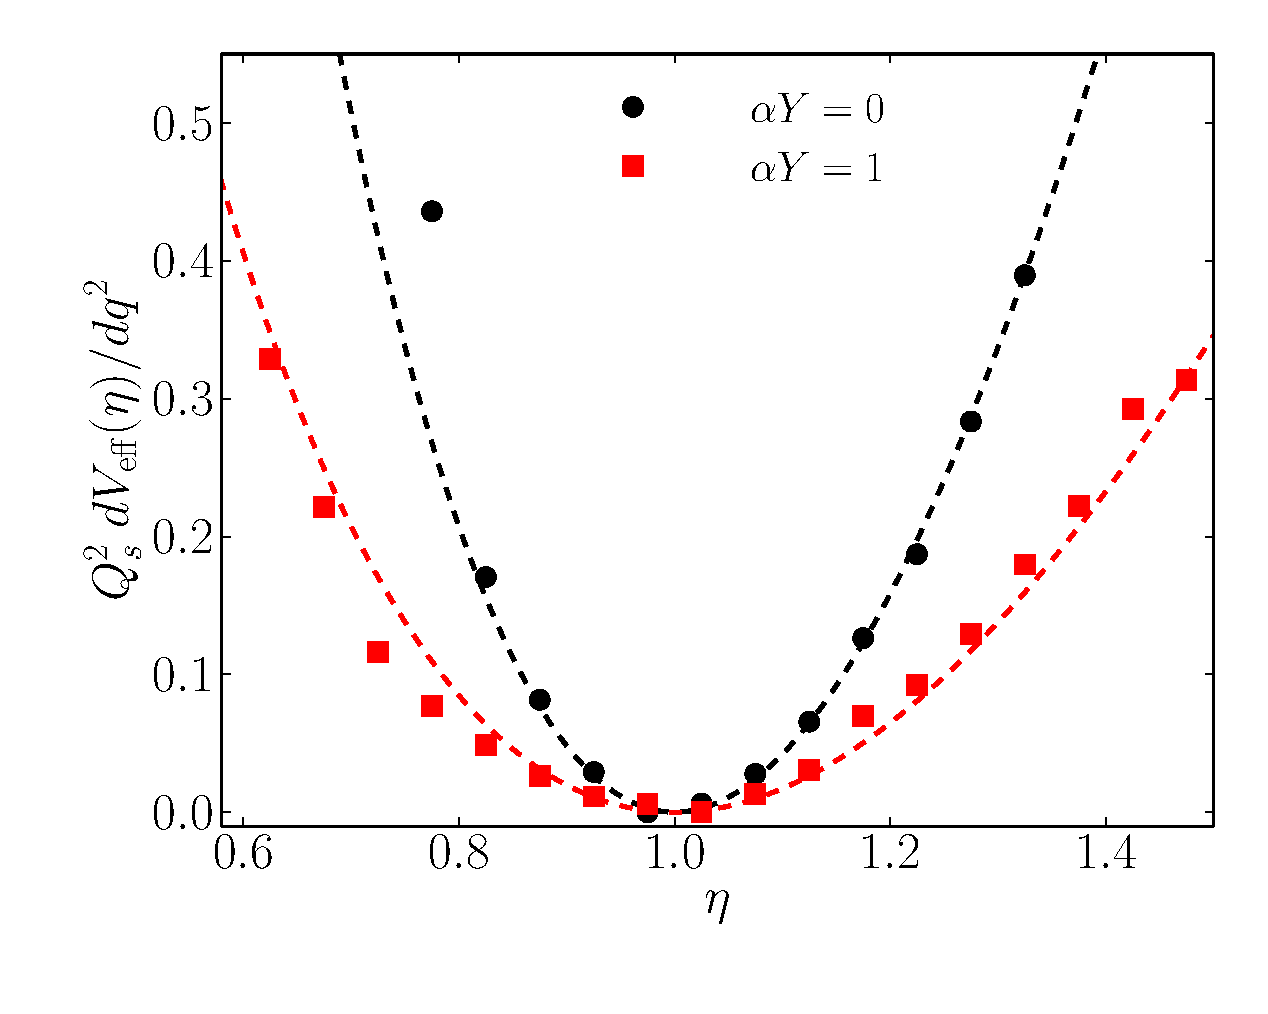
\includegraphics[width=\linewidth]{./figures/veff.pdf}
 }
\end{figure} 



Later, this effective theory was directly connected to 
the distribution of produced gluons in Ref.~\cite{Kovner:2018azs}. 
It turned out that the leading effect that drives the multiplicity 
fluctuations at small $x$ is the quantum Bose enhancement of gluons in the
proton wave function. Strikingly, from completely different presumptions,
the Liouville action was derived for the fluctuations of the effective saturation 
momentum~\cite{Iancu:2004es,Marquet:2006xm,Iancu:2007st}. 
In Refs.~\cite{Dumitru:2017cwt,Dumitru:2017ftq,Dumitru:2018iko} 
it was also realized that high multiplicity events at small $x$ 
cannot be parametrized by just a single  quantity  $Q_s$, 
but rather by a nontrivial function which depends on the transverse 
momentum and $x$. 

The systematic treatment of high multiplicity 
color charge configurations has only just begun and  
although this progress lead to a better understanding of the high multiplicity fluctuations, 
the state of the art numerical simulations in the saturation/CGC formalism 
(\cite{Mantysaari:2017cni,Mace:2018vwq,Mace:2018yvl} to name a few)
still rely 
on a brute force numerical approach to access high multiplicity tail. 
In this approach, configurations of target and projectile are generated 
without any bias, the particle production and correlations are computed and a posteriori 
multiplicity selection is applied. 
Given the numerical complexity of sampling these configurations  on a 2+1 dimensional lattice
(two transverse directions and rapidity),  
this approach  is very inefficient in probing 
high multiplicity tail, as most of the generated configurations are close to the most probable 
one. 

One of the goals of this proposal is to develop a theoretical high multiplicity ``trigger'', 
i.e. the reweighting technique providing  an efficient access to the high multiplicity tail.   

\subsubsection*{Small-x evolution}
Apart from the general advantage of having a semi-analytic solution, 
the dilute-dense expansion or knowing the function $f_i$ and $h_i$ (see Eqs.~\eqref{Eq:SIP} and~\eqref{Eq:DIP}) 
can facilitate the inclusion of small-$x$ evolution corrections~\cite{Kuraev:1977fs,
Balitsky:1978ic, 
Balitsky:1997mk, 
Balitsky:1998ya, 
Kovchegov:1999yj,
Kovchegov:1999ua, 
JalilianMarian:1997dw, 
JalilianMarian:1997gr,
Iancu:2001ad, 
Iancu:2000hn}.
Presently, in this framework,  the small-$x$ evolution has not been accounted for 
with rare exceptions and only
for single inclusive gluon production, see e.g. in Ref.~\cite{Dumitru:2018iko}. 
Usually, the dependence on $x$ is approximated by the IP-SAT model~\cite{Kowalski:2003hm,Rezaeian:2012ji},
which solves the leading order  DGLAP (Dokshitzer--Gribov--Lipatov--Altarelli--Parisi)  gluon evolution (neglecting its coupling to quarks) 
with analytically parametrized $x$ dependence at an initial 
transverse scale $\mu_0$. 
This approach provides a flexible and numerically simple method 
to the phenomenology. Nonetheless, incorporating actual non-linear 
small $x$ evolution is essential to study physics 
of high partonic densities and to extract phenomenological results from first principles.  
Doing so in the framework of JIMWLK (Jalilian-Marian--Iancu--McLerran--Weigert--Leonidov--Kovner) equation 
~\cite{JalilianMarian:1997dw, 
JalilianMarian:1997gr,
Iancu:2001ad, 
Iancu:2000hn} 
is one of the goals of this project. 
JIMWLK equation is a functional integro-differential 
equations describing evolution of the distribution of Wilson lines (or, alternatively, color sources) in a 
hadron. At the leading order, JIWMLK equations can be rewritten in the Fokker-Planck form~\cite{Weigert:2000gi}
and thus it can be also reformulated as  a Langevin equation describing a generalized Brownian motion of 
the Wilson line. Owing to its complexity, no analytic solution of the JIMWLK equation exists. 
Its solution has been obtained only numerically, using lattice gauge theory methods for the
 Langevin form of JIMWLK equation.

 At NLO, the JIMWLK equation does not allow for a straightforward reformulation in the Langevin form~\cite{Kovner:2014lca,Balitsky:2013fea}. 
 This is why the NLO JIMWLK equation has not been solved numerically yet. 	




Physically small $x$ evolution accounts for soft gluon emission and thus 
also contributes to multiplicity fluctuations. It is an open question how to 
incorporate high multiplicity ``trigger'' in small $x$ evolution (that is how to perform 
reweighting at each step of small $x$ evolution). 

%along with the running-coupling corrections [35–39] into the gluon production cross section.
%
%[35] E. Gardi, J. Kuokkanen, K. Rummukainen, and H. Weigert, Running coupling and power corrections in nonlinear
%evolution at the high-energy limit, Nucl. Phys. A784 (2007) 282–340, [hep-ph/0609087].
%[36] I. I. Balitsky, Quark Contribution to the Small-x Evolution of Color Dipole, Phys. Rev. D 75 (2007) 014001,
%[hep-ph/0609105].
%[37] Y. Kovchegov and H. Weigert, Triumvirate of Running Couplings in Small-x Evolution, Nucl. Phys. A 784 (2007)
%188–226, [hep-ph/0609090].
%[38] J. L. Albacete and Y. V. Kovchegov, Solving high energy evolution equation including running coupling corrections, Phys.
%Rev. D75 (2007) 125021, [0704.0612].
%[39] W. A. Horowitz and Y. V. Kovchegov, Running Coupling Corrections to High Energy Inclusive Gluon Production, Nucl.
%Phys. A849 (2011) 72–97, [arXiv:1009.0545].
%
%
%
%



\subsubsection*{Gluon saturation at Electron-Ion Collider} 
Because the final state effects are  minimal in e-A collisions, 
the small $x$ saturation/CGC framework can with greater effect be applied to 
quantifying particle scattering and production at an Electron-Ion Collider. 
At small $x$ Deep Inelastic Scattering (DIS) can be described in the so-called color 
dipole approach~\cite{Gunion:1976iy,Nussinov:1975mw,Nussinov:1975qb,Marquet:2009ca}: 
the virtual photon emitted by the incoming electron splits into quark and anti-quark.
This pair scatters off the target. The scattering is treated in the eikonal approximation.
These approach can be used for a wide variety of inclusive and semi-inclusive processes  
along with  smoking gun signatures of gluon saturation: suppression of dihadron 
correlations 
 and diffraction, in particular diffractive meson production 
(see most recent study in Ref.~\cite{Mantysaari:2017slo}
and Ref.~\cite{Aschenauer:2017jsk} 
for a comprehensive review). 



One of the processes which received our attention  is dijet (a jet pair) production in DIS.
And although in saturation/CGC formalism the color dipole approach is the most natural, 
it is important to mention, that in the correlations limit~\footnote{The correlation limit is  
the limit of almost back-to-back jets~\cite{Dominguez:2011wm,Dominguez:2011br}.}
it was shown that the saturation/CGC framework yields the same result for the dijet production
cross section as the one obtained within Transverse Momentum Dependent (TMD) factorization 
framework~\cite{Mulders:2000sh,Bomhof:2006dp,Meissner:2007rx} at small $x$~\cite{Metz:2011wb,Dominguez:2011wm}. 



Both approaches universally demonstrated that the dijet production depends on   
the Weiz\-s\"acker-Williams (WW) transverse-momentum-dependent  gluon distribution.  
The TMD parton distributions signify the recent progress achieved in developing 
frameworks to extend our understanding of hadron structure  beyond the one-dimensional
parton distribution function (PDF), as the TMDs depend not only of the longitudinal momentum 
fraction $x$ but also on the transverse momentum and therefore contain more 
detailed information on the internal structure of hadrons relative to PDFs.
Quark TMDs are the most studied, while the available studies of gluon TMDs 
are rather sparse. In particular, the WW gluon distribution still awaits its experimental 
determination; also theoretically little had been known about the evolution of the distribution at small $x$ 
before Ref.~\cite{Dumitru:2015gaa} where PI and coauthors conducted the first small $x$ computation of 
both components for the WW gluon distribution: unpolarized and polarized one, see Fig~\ref{fig:xGxh}. 
Both components can be accessed through measuring azimuthal anisotropies in processes 
such as dijet production in e+p and e+A scattering. The linearly polarized
gluon distribution causes  a nontrivial azimuthal angular $\cos 2\phi$ dependence of the dijet cross section, 
as we illustrate by the leading order in $\alpha_s$  cross-section for inclusive
production of a $q+\bar q$ dijet in high energy deep inelastic
scattering of a longitudinally~\footnote{The cross section for the transversely polarized virtual photon can be found in Refs.~\cite{Metz:2011wb,Dominguez:2011wm}.} polarized virtual photon $\gamma^*$ off a proton or nucleus is
given by~\cite{Metz:2011wb,Dominguez:2011wm}
\begin{eqnarray}
E_1E_2
\frac{d\sigma ^{\gamma _{L}^{\ast }A\rightarrow q\bar{q}X}}{d^3k_1d^3k_2 d^2b}
&=&\alpha _{em}e_{q}^{2}\alpha _{s}\delta \left( 1-z-\bar z\right) z^2\bar z^2\frac{8\epsilon _{f}^{2}{P}_{\perp }^{2}}{(
{P}_{\perp }^{2}+\epsilon _{f}^{2})^{4}}  %\notag \\
%&&
%\quad \quad \quad \quad \quad \quad
%\times
\left[ xG^{(1)}(x,q_{\perp })+\cos \left(2
  \phi\right)xh_{\perp }^{(1)}(x,q_{\perp })\right]\, .
\label{eq:dijet_L}
\end{eqnarray}
Here $\phi$ is the angle between the total momentum  ($P_\perp$) of dijet and the momentum imbalance  ($q_\perp$).
The feasibility of extracting the azimuthal anisotropy was 
consider in the proof of principle analysis of  Ref.~\cite{TODO}, where by doing Monte-Carlo simulations 
we showed that with some experimental effort the WW gluon distributions can
be successfully extracted, see Fig.~\ref{fig:extract}.

\begin{figure}[t]
\centering
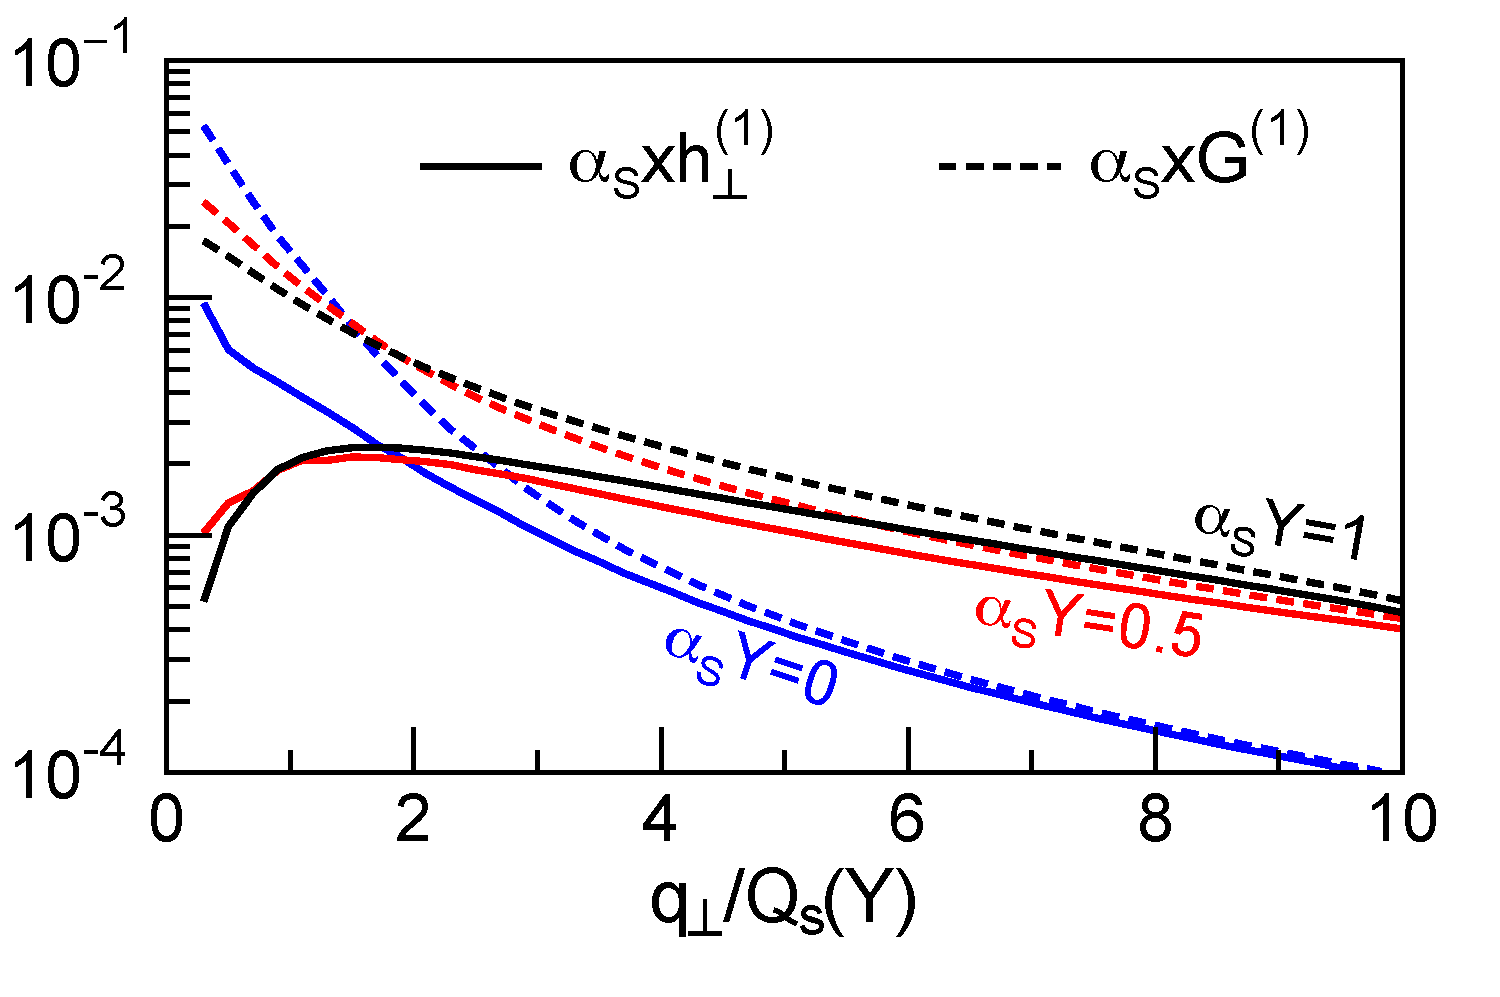
\includegraphics[width=0.45\linewidth]{figures/qs_multipl_log.pdf}
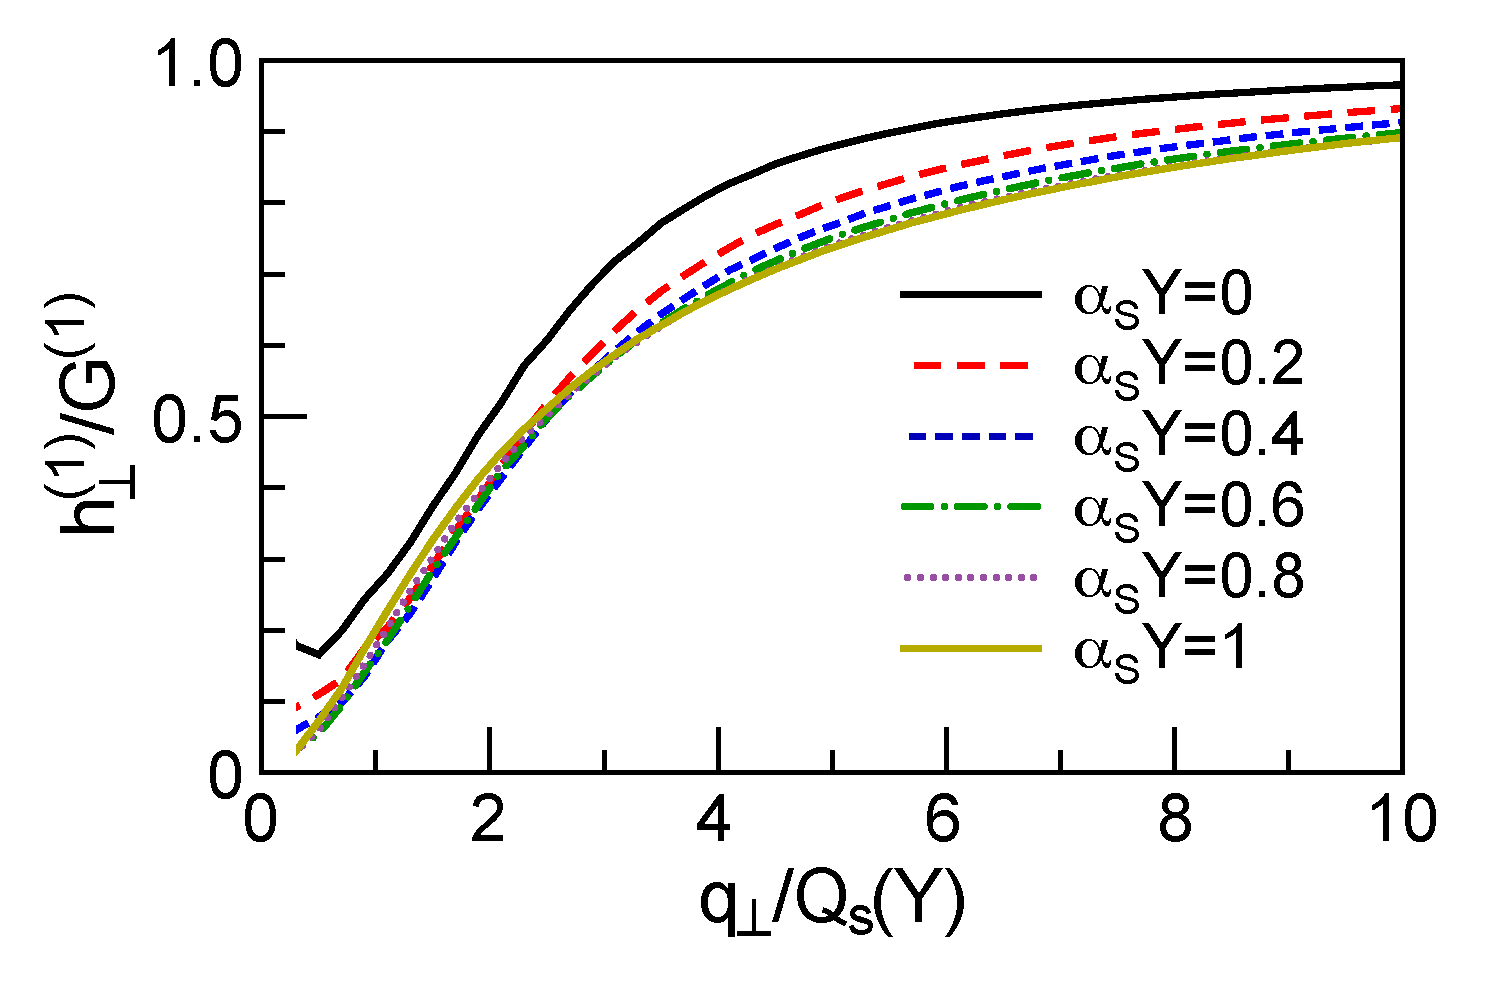
\includegraphics[width=0.45\linewidth]{figures/ratio.pdf}
%\vspace*{5cm}       % Give the correct figure height in cm
\caption{$xG^{(1)}(x,q^2_\perp)$ and $xh^{(1)}(x,q^2_\perp)$ WW gluon
  distributions versus transverse momentum $q_\perp$ at different rapidities
  $Y=\log x_0/x$. $Q_s(Y)$ is the saturation momentum. The computations are performed at 
  fixed $\alpha_s$~\cite{Dumitru:2015gaa}.
  The degree of gluon linear polarization is limited by the saturation of positivity bound and is maximal at high transverse momentum (dijet momentum imbalance). }
\label{fig:xGxh}       % Give a unique label
\end{figure}


\begin{figure}[b]

\floatbox[{\capbeside\thisfloatsetup{capbesideposition={right,top},capbesidewidth=8cm}}]{figure}
[0.8\linewidth]
%[\FBwidth]
{
\caption{Result of a fit of combined signal and background to a data sample obtained
	in $\sqrt{s}=90$ GeV $e$+A collisions with an integrated luminosity of 10 fb$^{-1}$/A.
	The results indicate that a proper measurement of
the linearly polarized gluon distribution will require integrated
luminosities of at least 20 fb$^{-1}$/A or more. Hence, this
measurement would be a multi-year program assuming that an EIC
initially starts off with luminosities around $10^{33}$ cm$^{-2}$
s$^{-1}$. See details in Ref.~\cite{TODO}
	}
	\label{fig:extract}
}
{ 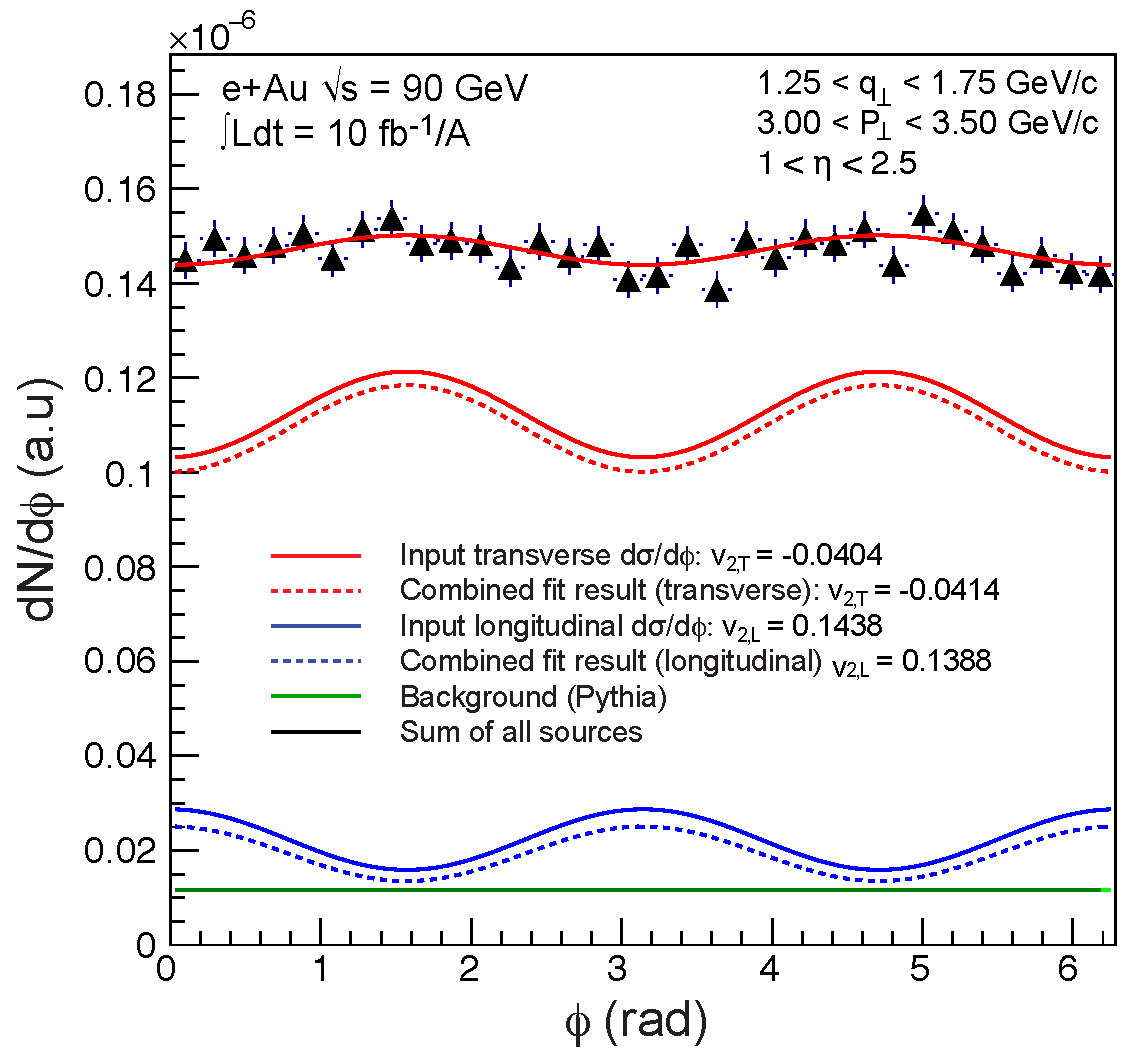
\includegraphics[width=\linewidth]{./figures/extract.pdf}
 }
\end{figure} 


{ 
	Small $x$ saturation/CGC formalism provides access to dijet production beyond the
	correlation limit~\cite{Dominguez:2011wm}; we illustrate this for the longitudinally 
	polarized virtual photon (c.f. Eq.~\eqref{eq:dijet_L}): 
	\begin{eqnarray}
&&\frac{d\sigma ^{\gamma_{L}^{\ast }A\rightarrow q\bar{q}X}}{d^2k_1dz_1d^2k_2dz_2}
= 8N_{c}\alpha _{em}e_{q}^{2} \, (2\pi)^2 \delta(1 -z- \bar{z}) 
z \bar{z} \epsilon_f^2
\int \frac{\text{d}^{2}u}{(2\pi)^{2}}\frac{\text{d}^{2}u^{\prime }}{(2\pi )^{2}}
\; e^{-i \v{P}\cdot(\v{u}-\v{u}^{\prime})}
 K_0(\epsilon_f u )   K_0(\epsilon_f u^\prime)  \\
&&~~~~\times 
\frac{1}{N_c}\left[
N_c+
\underbracket{
\left< {\rm Tr}\,
U^\dagger(\v{x_2})  U(\v{x_1}) U^\dagger(\v{x_1}^{\prime})  U(\v{x_2}^{\prime})
\right>_x}_{\rm quadrupole} 
-
\underbracket{\left< {\rm Tr}\,
U^\dagger(\v{x_2})  U(\v{x_1}) \right>_x}_{\rm dipole}
-
\underbracket{
\left< {\rm Tr}\,
U^\dagger(\v{x_1}^\prime)  U(\v{x_2}^\prime) \right>_x }_{\rm dipole}
\right] ~.  \label{Eq:disL} \notag
\end{eqnarray}
Here $\v{u}=\v{x_1}-\v{x_2}$ and $\v{u}^\prime=\v{x_1}^\prime-\v{x_2}^\prime$ and the angles represent averages over the 
target configurations. 
As we can see in Eq.~\eqref{Eq:disL},  the production cross section cannot be expressed in terms of  
	gluon TMDs but rather involve two- and four-point fundamental Wilson line ($U$) correlators (dipole and quadrupole terms)  in coordinate space. 
	Using the general saturation/CGC framework results,  we 
	estimated the amplitude of the azimuthal $\langle \cos 4\phi  \rangle$
	dependence in Ref.~\cite{Dumitru:2016jku}; it involved a new gluon TMD, i.e. it was not reducible to known gluon distribution. 
	Besides higher order harmonics, corrections to the correlation limit also 
	modify the angular independent amplitude and the amplitude of $\langle \cos 2\phi  \rangle$ anisotropy.
	This means that the corrections may also propagate to the observable azimuthal asymmetry.  
	They are controlled by the ratio $q_\perp^2/P_\perp^2$~\cite{Dumitru:2016jku}.    
	At an EIC, given statistical and collision energy limitations,  the kinematic range for the momentum imbalance and the 
	total dijet momentum is rather narrow; at best we could hope to get the ratio of $1/4$.
	This means that higher order corrections at an EIC can be phenomenologically important. 
	This necessitates numerical estimate of these corrections and implementation of the 
	full saturation/CGC formalism result, i.e. including the   full quadrupole contribution.   
	This is one of the aims of this proposal. 
	}




We note that similar structures involving dipole and quadrupole 
terms appear in single double inclusive production in the leading order of dilute-dense expansion in 
p-A and high multiplicity p-p collisions, see Eq.~\eqref{eq:SIPc} and the discussion on $h_1$ after 
Eq.~\eqref{Eq:DIP}. This illustrates an importance of a common framework to
particle production and scattering in 
p-p/A and e-A. 


Besides 
 extending and improving the dijet analysis, the application of the 
 developed framework to the smoking gun signatures of saturation in e-A collisions such as diffractive scattering/production
and dihadron correlations~\cite{Aschenauer:2017jsk} is also one of the goals of this project. 



\vspace{0.5em}
    \subsection{Detailed goals and methods}
        \label{sec:p11}

		Our main goal is to provide a unified systematic first-principle based description of
		initial-state effects and particle production/scattering in p-A, 
		high-multiplicity p-p, e-A and ultra peripheral p/A-A collisions.  
		The ultimate goal is to write and publish an open source  simulation code based on the same saturation/CGC framework and 
		the same set of parameters across different colliding systems. 

		The main milestones to be reached are listed below:
		\begin{itemize}
			\item Derivation of the first saturation correction to the leading order 
				dilute-dense approximation for single and double 
				inclusive gluon production, i.e. $f_2$ of Eq.~\eqref{Eq:SIP} and $h_2$  of Eq.~\eqref{Eq:DIP} correspondingly. 
				Previously PI with collaborators
				derived the momentum odd contribution to the double inclusive production, $h_2$, see Eq.~\eqref{Eq:DIP}, 
				in two different gauges: first in  the Fock-Schwinger gauge (this gauge is formulated in the coordinate space), see Ref.~\cite{McLerran:2016snu} and 
				then in the global light-cone gauge, see Ref.~\cite{Kovchegov:2018jun}.


				It may be straightforward, although technically difficult to derived complete 
				results for  $f_2$ and $h_2$ in the light-cone gauge. Thus, instead, 
				our approach will be based on the Fock-Schwinger gauge, where higher order corrections 
				can be obtained by iteratively solving classical Yang-Mills equation~\cite{Dumitru:2001ux,McLerran:2016snu}
				with appropriate boundary conditions~\cite{Kovner:1995ts}.
				The form of the result in the Fock-Schwinger gauge is usually the most convenient for 
				further numerical analysis on the lattice~\cite{Kovchegov:2018jun}.
				If we confront with unforeseen difficulties in the Fock-Schwinger gauge,
				we will be able to perform analytics in the light-cone gauge.  


				As was repeatedly pointed out  in Refs.~\cite{Mace:2018vwq,Mace:2018yvl}, the knowledge of the first saturation corrections, 
				$f_2$ and $h_2$, is required to estimate systematic uncertainties of the dilute-dense 
				approximation and, potentially, extend the range of applicability of the dilute-dense expansion to higher 
				gluon densities in the projectile. Also, higher order corrections may potentially reveal new non-trivial multi-gluon
				effects in two particle correlations patterns.  
			
				We will also  explore if higher order corrections, $f_2$ and $h_2$ can be written in approximately 
				$k_\perp$-factorized form as was previously done for te leading order dilute-dence expansion 
				of the double inclusive production~\cite{Kovchegov:2013ewa}.

			\item Developing reweighten for high multiplicity.  A posteriori multiplicity 
				selection is not well suited to probe extremely high multiplicity events. This necessitates 
				establishing an appropriate a priori reweighting
				techniques. Based on the insights we gained by computing gluon multiplicity distribution
				in a dilute  projectile~\cite{Dumitru:2017cwt,Dumitru:2017ftq,Dumitru:2018iko}, our  goal 
				is to  develop a reweighting which would  allow us to access the
				high-multiplicity tail; we will use this technique to compute multi particle correlations
				and nuclear modification factor.  

			\item Accounting for small $x$ evolution for particle production and correlations. 
				Application of the framework in the wide range of energies from RHIC and EIC to LHC, requires 
				inclusion of small $x$ evolution. The dilute-dense approximation allows straightforward 
				numerical implementation  of the evolution, which we will account for using leading order 
				JIMWLK equation. 

				Along with this we will consider two higher risk problems detailed below. 
				We want to stress that success of this project does not rely on solving these problems. 
				\begin{itemize}
					\item[--]
				We  plan to explore the possibility of reformulating NLO JIMWLK in the Langevin form and 
				solving it numerically. It is possible that the developed in this project reweighting method 
				will facilitate projection of each evolution step of LO JIMWLK to NLO order. This ideas are only 
				in its inception and will be considered in details during the implementation of this stage of the project.
					\item[--]
				From the result of Refs.~\cite{McLerran:2016snu,Kovchegov:2018jun}, it appears that 
				the presence of transverse momentum odd correlations in double inclusive production cross section 
				requires some degree of final state interactions (although 
				this statement may be gauge-dependent). It is thus important to understand if there
				are transverse momentum odd correlations in the {\it incoming} hadron wave function at small $x$
				before scattering and particle production. PI and collaborators  explored  this in an adhoc  JIMWLK motivated 
				wave function in Ref.~\cite{Kovner:2016jfp}; to improve  these calculations  we will consider 
				the hadron wave function derived from JIMWLK under controlled approximations.  
				\end{itemize}
			
			\item 
				Implementing the following key improvements to the Monte-Carlo dijet event generator (MCDijet) 
				for an EIC~\cite{TODO}:
				\begin{itemize}
					\item[--] incorporating event-by-event nucleon position fluctuations in nuclear target; 
					\item[--] studying correlations between dijet production and gluon multiplicity fluctuations 
						in the nuclear target; this might provide a realistic experimental probe 
						of WW gluon distribution in rare configurations of the nucleus/proton;
					\item[--] incorporating corrections to the correlation limit and simulations with complete 
						quad\-rupole contribution to dijet production; 
					\item[--] taking into account Sudakov corrections;  
					\item[--] probing model dependence with different color sources distributions 
						besides commonly used McLerran-Venugopalan (MV) model~\cite{McLerran:1993ni}. 
						Usually the initial condition for JIM\-WLK evolution are taken following 
						the MV model which is rigorously formulated only for large nuclei at 
						small $x$. For a proton at moderate and large $x$, the color charge 
						distribution can be quite different from the MV model. 
						As was shown in recent paper~\cite{Dumitru:2018vpr}, a
						standard light front Hamiltonian framework~\cite{Brodsky:1997de} can be used to compute color charge 
						distribution in nucleons and nuclei~\footnote{On the subject of light front quark model, 
							we will tap into expertise of a local nuclear theorist: Chueng-Ryong Ji.}  		
							; we want to implement this color distribution 
						to test model dependence of the results and provide a better estimates on 
						in dijet production at an EIC in a wide range on the targets' atomic number.    
				\end{itemize}
				These improvements are required in order to provide a realistic description of DIS
				dijet production at an EIC. 

				Additionally we plan to extend MCDijet to Ultra Peripheral Collision  (UPC) at hadron 
				colliders, such as RHIC and, especially, the LHC. 
				At very large impact-parameters between colliding hadrons the long range electromagnetic
				force becomes dominant over short-range QCD allowing for the dipole approach to 
				dijet production in UPC. One significant difference compared to DIS is that, for
				the UPC kinematics, the photon virtuality  is negligible; 
				this leads to vanishing amplitude in front of the linearly polarized gluon 
				distribution $x h^{(1)}_\perp$ (see e.g.~\cite{Dominguez:2011br}), 
				but the unpolarized gluon distribution, $xG^{(1)}$,  can be extracted. 
				We plan to conduct the realistic feasibility study of extracting  $xG^{(1)}$ in UPC 
				by 
				a) replacing the electron's photon fluxes with that from a proton or nucleus, as detailed in 
				Ref.~\cite{Klein:1999gv}
				and b) extending the range of accessible $x$ towards smaller values probed by  the LHC. 

				We also plan to modify MCDijet even generator to simulate the 
				suppression of dihadron correlations and diffractive meson production (beyond IP-SAT-based approach of Ref.~\cite{Toll:2012mb}). 	

			\item Application to phenomenology of p-p, p-A and e-A collisions. 
				In particular, we are interested in extracting the following observables 
				\begin{itemize}
					\item[--] Three-gluon correlations to explore if 
						the framework's systematics is similar to the STAR measurements
						in peripheral A-A collisions~\cite{Adamczyk:2017hdl,Adamczyk:2017byf}.  	
					\item[--] Four particle correlations and integrated and differential $v_n\{4\}$ as a function of  multiplicity and collision energy
					\item[--] Nuclear modification factor with multiplicity bias, so-called $Q_{pA}$~\cite{Adam:2014qja}.  
					\item[--] 
					Systematics of Dijet Production at an EIC and UPC: 
					dependence on the atomic number, energy dependence, 
					prediction for high order harmonics of azimuthal anisotropy, 
					feasibility check of extracting correlation between dijet production and forward nucleus going  multiplicity, as a probe of biased WW gluon distribution, cristalysing the role of saturation in dijet observables.  
				\end{itemize}
		\end{itemize} 
		
		
		
%		The PI has experience in writing, publishing and maintaining source code, see e.g. MCDijet~\cite{ }.




    \vspace{0.5em}
    \subsection{Timeline}
        \label{sec:p12}
The targeted due dates for the deliverables are indicated in quarter year
increments: e.g., Q4 refers to delivery one year after the project funding
begins, and Q12 refers to the end of the three-year project.

%{\TODO update}
        \begin{enumerate}
            \item Tasks oriented towards e-p/A and  
				ultra-peripheral p-A and A-A collisions   
                \begin{itemize}
                    \item Extension of MCDijet,  Monte-Carlo generator 
						for dijet production, to UPC (Q6)
                        \begin{itemize}
                            \item Extending small $x$ evolution to cover 
								LHC energy range, incorporating running
								coupling corrections  (Q2)
                            \item Incorporating nucleon position fluctuations 
								in nuclear wave function (Q4)
                            \item Publishing the even generator MCDijet for UPC  (Q6)
                        \end{itemize}
                    \item Rare nuclear wave function configurations 
						and dijet production 
						(Q8)
                        \begin{itemize}
							\item Light front quark model for 
							nucleon wave function in e-p collisions (Q2) 
                            \item Incorporating nucleon position fluctuations 
								in nuclear wave function   (Q3)
                            \item Inclusion of Sudakov corrections and
								estimating their importance  (Q6)
                            \item   
								Complete quadrupole contribution to dijet production  (Q8)
                        \end{itemize}
                \end{itemize}
        \end{enumerate}
        \begin{enumerate}
            \item  Tasks oriented towards p-p 
				and  p-A  collisions  
                \begin{itemize}
                    \item Theoretical development for p-A collisions (Q10)
                        \begin{itemize}
                            \item Complete result for single and double 
								gluon production with first saturation 
								correction (Q4)
                            \item High-multiplicity reweighting  (Q10)
                        \end{itemize}
                    \item Numerical simulations and publishing the final version 
					of the 	code (Q12)
                        \begin{itemize}
                            \item Role of complete first saturation correction on 
								event-by event number of gluon distribution 
								and on even harmonics, $v_{2n}$ (Q5)
                            \item Inclusion of small-x evolution  (Q7)
                            \item Numerical simulations with
								high multiplicity trigger (Q11)
							\item Application to phenomenology (Q1-Q12)
							\item GPU-based implementation of the code (Q12) 
                        \end{itemize}
                \end{itemize}
        \end{enumerate}

% Section 2
\section{Proposed Research: Entanglement and full density matrix}
    \label{sec:p2}

    \vspace{0.5em}
    \subsection{Background}
    \label{sec:p2b}

momentum enrangelement -- small - large x 



    \vspace{0.5em}
    \subsection{Detailed goals and methods}
        \label{sec:p21}
The main motivation for these ramblings is the idea that one should be able to get some idea about correlation
between the profile of the charge density and the current density in the hadronic wave function at high energy. One
may expect for example, that if the scattering catches a configuration with large density or large density gradient,
this configuration will naturally also have a large current, since it does not want to stay static for a long time. The
large current then may translate into relatively high momenta of the particles in the wave function. That way we
may be able to relate on the level of the initial hadronic state the density (number)
fluctuation in the configuration
space and momentum distribution of particles.


Evolution of entangelement entropy 


    \vspace{0.5em}
    \subsection{Timeline}
        \label{sec:p22}
  \item Momentum entanglement in hadronic wave function
        \begin{enumerate}
            \item Full density matrix  in the basis 
				of valence charge density
                \begin{itemize}
                    \item Small-$x$ evolution of full density matrix (Q6)
                        \begin{itemize}
                            \item Deriving evolution equation (Q2)
                            \item Gaussian approximation and application to small-$x$ 
								phenomenology (Q4)
                            \item Relation to high-multiplicity events and correlation between large and small x components of the hadronic  wave function (Q6)
                        \end{itemize}
                    \item  Small-$x$ evolution of entangelment entropy   (Q10)
                        \begin{itemize}
                            \item Deriving small-$x$ evolution (Q7)
                            \item Solving small-$x$ evolution on lattice (Q8)
                            \item Phenomenological application  (Q10)
                        \end{itemize}
                \end{itemize}
        \end{enumerate}

% Section 3
\section{Proposed Research: Quantum statistics at small $x$}
    \label{sec:p3}

    \vspace{0.5em}
    \subsection{Background and motivation}
    \label{sec:p3b}
	Although the quantum statistic effects are exuberant at small $x$, 
	only recently their significance was recognized in observables. 
	In particular, 
	for gluons, three sources of multi-particle  correlations were rigorously established at 
	small $x$: -- Bose Enhancement, -- Hanbury Brown-Twiss (HBT), and classical effects due to 
	scattering off a domain with spontaneous rotational symmetry breaking of the direction of 
	color field~\cite{Dumitru:2014yza,Dumitru:2014vka,Dumitru:2015cfa}. It was shown that two genuinely quantum effects dominate over the classical one 
	almost in the entire phenomenologically relevant kinematic range~\cite{Kovner:2018azs}.
	Specifically, it was demonstrated that the ridge correlations at small $x$ are 
	due mostly to gluon Bose enhancement and 
	HBT~\cite{Kovchegov:2013ewa,Kovchegov:2012nd,Altinoluk:2015uaa,Altinoluk:2018ogz,Kovner:2018fxj,Kovchegov:2018jun};
	also  it was recently identified 
	that gluon Bose enhancement is responsible for the high multiplicity tail in p-A collisions~\cite{Kovner:2018azs}. 
	Finally, it was shown that Fermi statistics my lead to non-trivial effects at small $x$~\cite{Altinoluk:2016vax,Kovner:2017ssr,Kovner:2018vec} 
and potentially be responsible for a significant background contribution to the Chiral Magnetic Effect~\cite{Kovner:2017gab}. 
	The latter was established only on the level of particle correlations in the incoming projectile wave function; 
	quite recently the saturation/CGC framework applied to derive semi-analytic equations describing 
	three particle correlations, including the CME observable~\cite{Martinez:2018tuf}. Numerical calculations of this 
	correlations has not yet been performed and currently we can only speculate how large 
	this contribution is in p-A and A-A collisions. One of the goals of this project is to 
	numerically extract CME correlator in dilute-dense saturation/CGC framework and to asses its phenomenological importance 
	for CME studies. 

	Quantum statistics might be responsible not only for the intriguing observation of three particle CME-like correlations 
	in p-A collisions, but also for an observed near-side baryon--baryon anti-correlation structure in p-p 
	collisions~\cite{Adam:2016iwf} at the LHC. Currently the description of this effect presents a challenge 
	to all Monte Carlo models and its origin is an open question. Exploratory studies to probe if this anti-correlations are 
    related to parton statistics at small $x$ will be conducted in project.  


	


    \vspace{0.5em}
    \subsection{Detailed goals and methods}
        \label{sec:p31}

		Here, the main goal is to elucidate the role of quantum statistics effects at small $x$ by 
		conducting analytical and numerical analysis of quark and gluon production and correlations. 
		The main milestones are 
		\begin{itemize}
			\item By conducting 
				numerical simulation of deuteron-A collision 
				on the lattice, test the hypothesis that high multiplicity tail is dominated by 
				configurations of the deuteron with the overlapping nucleons in the transverse direction~\cite{Kovner:2018azs,Mace:2018vwq}. 
				The foundation of this hypothesis is based on gluon Bose enhancement in the projectile~\cite{Mace:2018vwq}.   
			\item Implementing a realistic wave function for the {\it polarized} deuteron. 
				Due to an admixture of the 
				$D$-wave state in the deuteron wave function (see e.g. \myref\cite{Machleidt:2000ge}), 
				the direction of deuteron polarization defines the spatial
				anisotropy of deuteron. Thus polarized deutron-nucleus collisions 
				at high energy provide a unique system for measuring effects of quantum statistics sensitive to the 
				deuteron wave function including Bose enhancement and HBT. Additionally  the polarized deuteron collisions 
				provide the knowledge of the initial eccentricity and a good handle on the reaction plane orientation; 
				this may facilitate disentangling and testing the role of initial and final state effects in driving
				azimuthal anisotropy in d-A collisions.
			\item  Testing  numerically the saturation/CGC predictions in polarized d-A collisions, in particular: -- that  the longitudinal 
				deuteron polarization leads to greater multiplicity fluctuations than the transverse deuteron polarization,  --  that 
				two gluon correlations are stronger along the axis polarization due to gluon HBT. Assessing if this effect can be experimentally
				measured.
			\item Implementing quark production in the framework. Applying the framework to extract numerically: -- 
				the background contribution to the Chiral Magnetic Effect, i.e. the three particle charge-dependent correlator, -- 
				the quark--quark and quark--anti-quark correlation function and explore if it may be responsible for the 
				observed baryon-baryon rapidity anti-correlation. 
			\item Providing a realistic 
				initial baryon number  distribution in the coordinate space for further hydrodynamic evolution in A-A collisions. 
		\end{itemize}
		
		
		Summarizing the above research complemented by that conducted previously, 
		we plan to write a comprehensive review on the quantum statistics effects at small $x$. 


    \vspace{0.5em}
    \subsection{Timeline}
        \label{sec:p32}
        \begin{enumerate}
            \item Exploring role of quantum statistics at small $x$
                \begin{itemize}
                    \item Investigating the role of gluon quantum statistics (Q8)
                        \begin{itemize}
                            \item Numerical simulations of unpolarized deuteron-A collisions: role of Bose enhancement (Q2) 
                            \item Polarized deuteron wave function and two gluon correlations as a test of quantum 
								statistics effects and collectivity (Q8) 
                        \end{itemize}
                    \item Investigating the role of quark statistics (Q10)
                        \begin{itemize}
                            \item Implementing quark degrees of freedom in numerical simulations (Q5)
                            \item Computing two and three particle correlations involving quark degrees of freedom (Q8)
                            \item Computing tables of the initial baryon number distribution for further hydrodynamical evolution in A-A collisions   (Q10)
                        \end{itemize}
                \end{itemize}
        \end{enumerate}



    
    
    % Extras
  %  \section{Project Management Plan}
  %     \label{sec:management}
  %    \lipsum[91-100]




  %  \section{Software Productivity and Sustainability Plan}
  %      \label{sec:software_sustainability}
  %      \lipsum[111-120]



    % end of proposal narrative
    
		\vspace{1em}
    \section*{\underline{End of proposal narrative; supplemental materials to follow.}}
    \newpage


    % supplemental materials
    \addcontentsline{toc}{section}{Supplemental Materials:}
    
	    \section{Data Management Plan}
        \label{sec:data_management}
        
We will follow the below protocol: 
\begin{itemize}

	\item 
The published data will be distributed as  supplementary  material for each 
published manuscript in a widely used format, e.~g. 
ASCII or tab-delimited  format. 
Instructional material will be provided in 
the manuscripts and in text form along  with the data. 
The data will be strictly in standard, non-proprietary file formats 
to facilitate  data sharing. 

\item 
For each published manuscript, in case of large data files, 
the PI will make copies of data 
available to co-investigators, students, and
others by request within 30 days of receipt of the request. 
 


	\item
The simulation code will be developed in C++, Python and Julia, 
the data processing  scripts will be written using sed and awk. 
Every piece of written software or script will 
be provided to the public in source code format for non-commercial use 
under GNU General Public License (GPL). 
For each code made available, a user's manual will be provided with
instructions for compiling the source codes, installing and running the codes,
formulating input data streams, and visualizing the output. Documentation will
be in PDF format.
Source codes will be published on the North Carolina State University 
	GitHub web page \url{https://github.ncsu.edu}. 

\item 
For all of the numerical simulations, representative input files will
be kept along with the sources codes. Sample  output files 
will also be provided when possible. 

\end{itemize}

	\newpage 

	
	\section{Student Tracking Information}
        \label{sec:staffing}
        \vspace{0.5em}

\begin{center}
\begin{tabular}{| p{16mm}| p{25mm}| p{22mm}| p{18mm}|p{25mm}|p{15mm}|  }                                                                              \hline
             Student & Date~Entered Grad. School  &   Date Joined Group & Degree Program 
			 & Date Degree Expected & Advisor \\
            \hline
             Gregory Johnson & August 2017 & July 2018  & Ph.D.  & May 2022  & Skokov \\ 
			 \hline
             Haowu Duan &  August 2017    & August 2018  & Ph.D.   & May 2022 & Skokov \\ 
			 \hline
        \end{tabular}

\end{center}
%\lipsum[121-130]

    \newpage

  %  \section{Project Timeline}
  %      \label{sec:timetable}
   %     The targeted due dates for the deliverables are indicated in quarter year
increments: e.g., Q4 referes to delivery one year after the project funding
begins, and Q12 referes to the end of the three-year project.


%stuff to make enumerate mimic section numbering:
\renewcommand{\labelenumii}{\arabic{enumi}.\arabic{enumii}}
\renewcommand{\labelenumiii}{\arabic{enumi}.\arabic{enumii}.\arabic{enumiii}}
\renewcommand{\labelenumiv}{\arabic{enumi}.\arabic{enumii}.\arabic{enumiii}.\arabic{enumiv}}

\begin{enumerate}
\setcounter{enumi}{0} %start on sect 2 for consistency w/ section labeling.

    \item Build a unified framework for a systematic first-principle 
		description of multiparticle production and multiparticle 
		correlations at small $x$ in various colliding systems
        \begin{enumerate}
            \item Tasks oriented towards e-p/A and  
				ultra-peripheral p-A and A-A collisions   
                \begin{itemize}
                    \item Extension of MCDijet,  Monte-Carlo generator 
						for dijet production, to UPC (Q6)
                        \begin{itemize}
                            \item Extending small $x$ evolution to cover 
								LHC energy range, incorporating running
								coupling (Q2)
                            \item Incorporating nucleon position fluctuations 
								in nuclear wave function (Q4)
                            \item Publishing MCDijet for UPC  (Q6)
                        \end{itemize}
                    \item Rare nuclear wave function configurations 
						and dijet production 
						(Q8)
                        \begin{itemize}
							\item Light front quark model for 
							nucleon wave function in e-p collisions  
                            \item Incorporating nucleon position fluctuations 
								in nuclear wave function   (Q3)
                            \item Sudakov  (Q6)
                            \item Beyond correlation limit  (Q8)
                        \end{itemize}
                \end{itemize}
        \end{enumerate}
        \begin{enumerate}
            \item  Tasks oriented towards p-p 
				and  p-A  collisions  
                \begin{itemize}
                    \item Theoretical development for p-A collisions (Q10)
                        \begin{itemize}
                            \item Complete result for single and double 
								gluon production with first saturation 
								correction (Q4)
                            \item High-multiplicity reweighting  (Q10)
                        \end{itemize}
                    \item Numerical simulations and publishing the final version 
					of the 	code (Q12)
                        \begin{itemize}
                            \item Role of complete first saturation correction on 
								event-by event number of gluon distribution 
								and on even harmonics, $v_{2n}$ (Q5)
                            \item Inclusion of small-x evolution  (Q7)
                            \item Numerical simulations with
								high multiplicity trigger Q(11)
                        \end{itemize}
                \end{itemize}
        \end{enumerate}

    \item Momentum entanglement in hadronic wave function
        \begin{enumerate}
            \item Full density matrix  in the basis 
				of valence charge density
                \begin{itemize}
                    \item Small-$x$ evolution of full density matrix (Q6)
                        \begin{itemize}
                            \item Deriving evolution equation (Q2)
                            \item Gaussian approximation and application to small-$x$ 
								phenomenology (Q4)
                            \item Relation to high-multiplicity events and correlation between large and small x components of the hadronic  wave function (Q6)
                        \end{itemize}
                    \item  Small-$x$ evolution of entangelment entropy   (Q10)
                        \begin{itemize}
                            \item Deriven small-$x$ evolution (Q7)
                            \item Solving small-$x$ evolution on lattice (Q8)
                            \item Phenomenological application  (Q10)
                        \end{itemize}
                \end{itemize}
        \end{enumerate}
        \begin{enumerate}
            \item Exploring role of quantum statistics at small $x$
                \begin{itemize}
                    \item Major task 3 (Q6)
                        \begin{itemize}
                            \item Minor Task 1 (Q2)
                            \item Minor Task 2 (Q4)
                            \item Minor Task 3 (Q6)
                        \end{itemize}
                    \item Major task 4 (Q12)
                        \begin{itemize}
                            \item Minor Task 4 (Q5)
                            \item Minor Task 5 (Q10)
                            \item Minor Task 6 (Q12)
                        \end{itemize}
                \end{itemize}
        \end{enumerate}

\end{enumerate}


   % \newpage


    % The bibliography 
   % \section{Abbreviations and Code Names}
   %     \label{sec:abbreviations}
   %     \begin{tabular}{p{1.0in}p{5.4in}}
    ACME & Accelerated Climate Model for Energy (both code and project) \\
    ACME v0 & Version 0.0 of ACME model, 2014 \\
    ACME v1 & Version 1.0 of ACME model, 2016 \\
    ACME v2 & Version 2.0 of ACME model, ~2018 \\
\end{tabular}

   % \newpage

	\newpage 
    \section{Literature Cited} 
	{%\fontsize{10}{10}\selectfont
		\label{sec:references}
        \bibliography{bibl,references,v3}
	}
    \newpage

	\section{List of Principle Collaborators}
        \label{sec:PC}
        %\begin{document}
\vspace{0.5em}
\noindent
{\bf  \Investigator: }


{
\it
\noindent
Bzdak, Adam (AGH-UST), \\
Dumitru, Adrian (Baruch College),\\
Friman, Bengt (GSI),\\
Fukushima, Kenji (Tokyo Uni),\\ 
Kharzeev, Dmitri (SBU),\\
Koch, Volker (LBNL),\\
Kovchegov, Yuri (OSU),\\
Kovner, Alex (UConn),\\
Lappi, Tuomas (Jyvaskyla Uni),\\
Levai, Peter (Wigner Institute),\\ 
Lublinsky, Michael (Ben Gurion U. of Negev), \\
Mace, Mark (BNL),\\
McLerran, Larry (INT),\\ 
Nakano, Eiji (Kochi Uni),\\
Nishimura, Hiromichi (RBRC),\\
Pisarski, Robert (BNL), \\
Redlich, Krzysztof (Wroclaw),\\
Tribedy, Prithwish (BNL), \\
Ullrich, Thomas (Yale), \\
Venugopalan, Raju (BNL)
}

    \newpage

    % The short biosketches for EVERY contributing person
 
	
	\section{Biographical Sketches}
        \label{sec:biosketches}
        
%The following pages list 2-page CVs for the key personnel listed below.

%\begin{itemize} \zapspace
%    \item{\Investigator}
%\end{itemize}

%\newpage

% NOTE: You can import tex bios like so
%\newpage

\begin{center}
   {\large\bf Vladimir Skokov} \\[0.25em]
    Physics Department, College of Sciences \\
    North Carolina State university, Raleigh, NC 27695 \\
    Email: vskokov@ncsu.edu
\end{center}

\noindent\textbf{Education and Training}

\vspace{0.6em}
\begin{tabular}{rp{5.6in}}
	2006 & Ph.D., Physics, Joint Institute for Nuclear Researchers, Dubna, Russian Federation \\[0.5em]
	2002 & M. Sc., Physics, Saratov State University \& Joint Institute for Nuclear Researchers, Russian Federation \\[0.5em]
\end{tabular}
\vspace{0.6em}
    
\noindent\textbf{Research and Professional Experience}

\vspace{0.6em}
\begin{tabular}{lp{5in}}
    {2018--present} & Assistant Professor, 
	North Carolina State University, 
	Raleigh, NC. \\[0.5em]
    {2018--present} & Fellow, 
	Riken-BNL Research Center, 
	Brookhaven National Laboratory, 
	Upton, NY. \\[0.5em]
    {2015--2018} & Research Associate, 
	Riken-BNL Research Center, 
	Brookhaven National Laboratory, 
	Upton, NY. \\[0.5em]
    {2013--2015} & Visiting Assistant Professor (non-tenure), 
	Western Michigan University, 
	Kalamazoo, MI.  \\[0.5em]
    {2011--2013} & Research Associate, 
	Physics Department, 
	Brookhaven National Laboratory, 
	Upton, NY. \\[0.5em]
    {2009--2011} & Research Associate, 
	GSI Helmholtzzentrum fuer Schwerionenforschung, 
	Darmstadt, Germany. \\[0.5em]
\end{tabular}

\vspace{0.6em}

\noindent\textbf{Awards} % Top 10!
\begin{itemize}
	\item[] {\it Fellowship}\\ 
		2012, 2017, 2018  EMMI Research Visiting Professor GSI, Darmstadt, Germany
	\item []  {\it Fellowship}\\ 	
		2003, 2005 Bogoliubov-Infeld Fellowship, JINR, Dubna, Russia
	\item []  {\it Fellowship} 	\\ 
		2001 Leonard Euler Fellowship, Justus-Liebig-Universitaet, Giessen, Germany
	\item []  {\it Fellowship} 	\\ 
		2000 CRDF Grant for Undergraduate Scientific Research, Saratov State
University,  Russia
\end{itemize}

\vspace{0.6em}

\noindent\textbf{Selected Publications} % Top 10! 
\\
\noindent{\it Most pertinent publications for the past three years} % Top 10!

\begin{itemize}
	\setlength\itemsep{0.25em}	
	\item[]  
		M.~Mace, V.~Skokov, P.~Tribedy and R.~Venugopalan, \\
  ``Hierarchy of azimuthal anisotropy harmonics in collisions of small systems from the Color Glass Condensate,'' \\
  \href{http://dx.doi.org/10.1103/PhysRevLett.121.052301}{
	  Phys.\ Rev.\ Lett.\  {\bf 121}, no. 5, 052301 (2018)}

  \item[]
		A.~Kovner and V.~Skokov, \\
	   ``Does shape matter? $v_2$ vs eccentricity in small x gluon production'', \\ 
	   \href{https://doi.org/10.1016/j.physletb.2018.09.001}{
 	Phys.\ Lett.\ B {\bf 785}, 372 (2018)}


	\item[]   
		A.~Kovner and V.~Skokov, \\
  ``Bose enhancement, the Liouville effective action and the high multiplicity tail in p-A collisions,'' \\
  \href{http://dx.doi.org/10.1103/PhysRevD.98.014004}{ 
  Phys.\ Rev.\ D {\bf 98}, no. 1, 014004 (2018)}

	\item[]   
		Y.~V.~Kovchegov and V.~Skokov, \\
  ``How classical gluon fields generate odd azimuthal harmonics for the two-gluon correlation function in high-energy collisions,'' \\
  \href{http://dx.doi.org/doi:10.1103/PhysRevD.97.094021}  {
	  Phys.\ Rev.\ D {\bf 97}, no. 9, 094021 (2018) }

	\item[]  
		A.~Dumitru, G.~Kapilevich and V.~Skokov,\\
  ``The small-x gluon distribution in centrality biased pA and pp collisions,''\\
  \href{http://dx.doi.org/doi:10.1016/j.nuclphysa.2018.03.012}{
	  Nucl.\ Phys.\ A {\bf 974}, 106 (2018)}


	\item[] 
		A.~Kovner, M.~Lublinsky and V.~Skokov,\\
  ``Initial state qqg correlations as a background for the Chiral Magnetic Effect in collision of small systems,''\\
  \href{http://dx.doi.org/doi:10.1103/PhysRevD.96.096003}{
	  Phys.\ Rev.\ D {\bf 96}, no. 9, 096003 (2017)}

  \item[] 
	  A.~Dumitru and V.~Skokov,\\
  ``Fluctuations of the gluon distribution from the small-x effective action,''\\
   \href{http://dx.doi.org/doi:10.1103/PhysRevD.96.056029}{
  Phys.\ Rev.\ D {\bf 96}, no. 5, 056029 (2017)
}

  \item[]
	   A.~Kovner, M.~Lublinsky and V.~Skokov,\\
  ``Exploring correlations in the CGC wave function: odd azimuthal anisotropy,''\\
   \href{http://dx.doi.org/doi:10.1103/PhysRevD.96.016010}{
  Phys.\ Rev.\ D {\bf 96}, no. 1, 016010 (2017)
}

  \item[]
	    L.~McLerran and V.~Skokov,\\
  ``Odd Azimuthal Anisotropy of the Glasma for pA Scattering,''\\
   \href{http://dx.doi.org/doi:10.1016/j.nuclphysa.2016.12.011}{
Nucl.\ Phys.\ A {\bf 959}, 83 (2017)
}
  \item[]
	    A.~Dumitru and V.~Skokov,\\
  ``$cos(4 \phi )$ azimuthal anisotropy in small-$x$ DIS dijet production beyond the leading power TMD limit,''\\
   \href{http://dx.doi.org/doi:10.1103/PhysRevD.94.014030}{
  Phys.\ Rev.\ D {\bf 94}, no. 1, 014030 (2016)
}

	\item[]
    A.~Dumitru, T.~Lappi and V.~Skokov,\\
  ``Distribution of Linearly Polarized Gluons and Elliptic Azimuthal Anisotropy in Deep Inelastic Scattering Dijet Production at High Energy,''\\
  \href{http://dx.doi.org/doi:10.1103/PhysRevLett.115.252301}{
  Phys.\ Rev.\ Lett.\  {\bf 115}, no. 25, 252301 (2015)
  }

  \item[]
	    A.~Dumitru, L.~McLerran and V.~Skokov, \\ 
		``Azimuthal asymmetries and the emergence of “collectivity” from multi-particle correlations in high-energy pA collisions,''\\
		\href{http://dx.doi.org/doi:10.1016/j.physletb.2015.02.046}{
			Phys.\ Lett.\ B {\bf 743}, 134 (2015)}
\end{itemize}






% NOTE: But, You'll probably import PDF versions of everyones short CV like so
%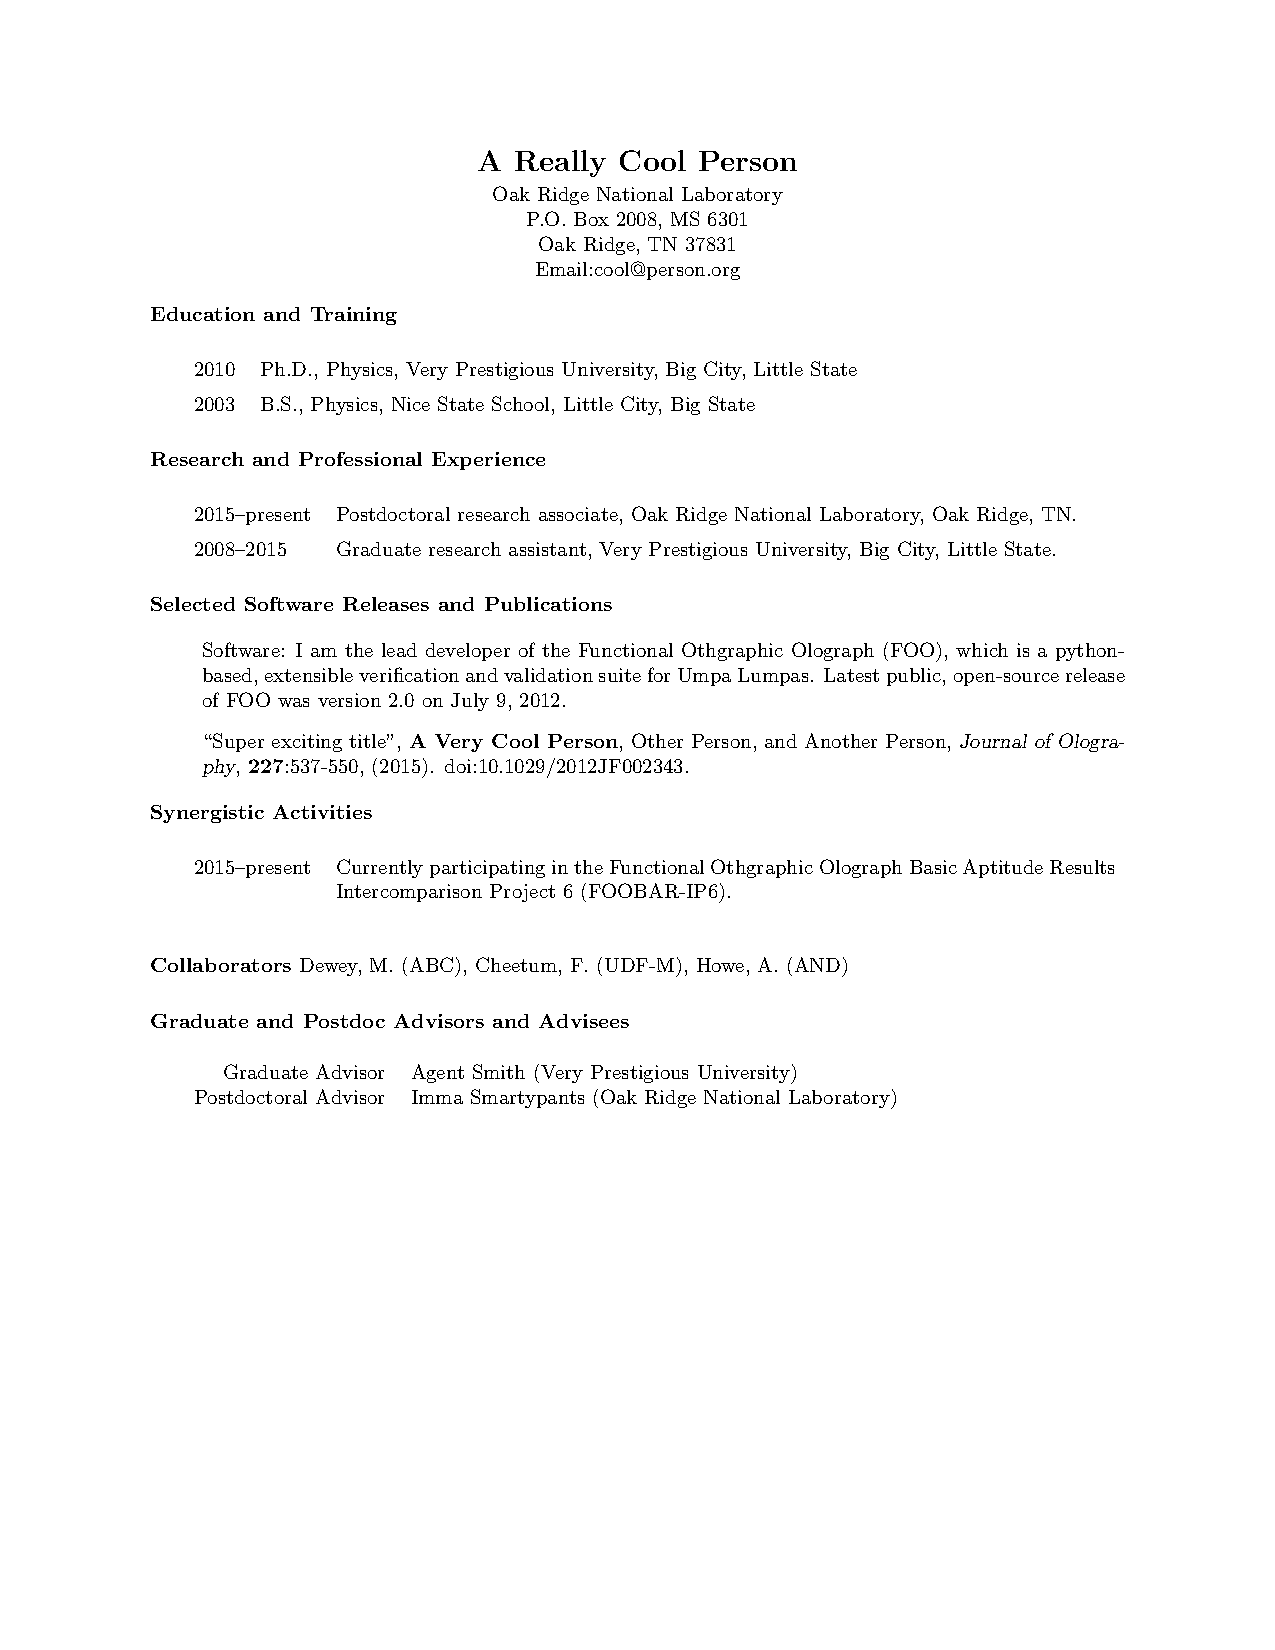
\includepdf[pages=-,pagecommand={\thispagestyle{plain}}]{Bios/cv_example.pdf}


    
	\newpage 
	\section{Current and Pending Support}
        \label{sec:grants}
	
	{\bf Current Support}

	\noindent
	Title: BEST
	
	\noindent
	Principal Investigator: ???  


	\newpage 
	\section{Facilities and Resources}
        \label{sec:facres}
	
		The work will be mainly conducted at North Carolina State University. 


		The PI joined 
		the nuclear theory group at North Carolina State University, which consists
		of Chueng-Ryong Ji, Thomas Sch\"afer, and Mithat \"Unsal. 
		North Carolina State also has a strong representation in	
		nuclear astrophysics, led by Carla Fr\"ohlich, Gail McLaughlin,
		and Jim Kneller. 
		The groups collaborate with the Nuclear Theory Groups 
		at Duke  and the University of North
		Carolina at Chapel Hill. 
		The nuclear theory faculty at Duke includes Steffen Bass, 
		Shailesh Chandrasekharan, Tom Mehen, and Roxanne Springer. 
		The theory group at UNC Chapel Hill consists of Jon Engel, Joaquin Drut and Amy Nicholson.
		
		The  NCSU Nuclear Theory group has access to the computing capabilities of  
		North Carolina State University, which   
		maintains \href{https://projects.ncsu.edu/hpc//main.php}{High Performance Computing} 
		cluster. The cluster has 1344 computes nodes (mostly dual Xeon), 
		over 11000 cores, 2-4GB per core distributed memory, and 10Gb Ethernet interconnects.
		GPU (NVIDIA) nodes are available. 
		The cluster provides 1TB mass storage space per project. 
		The PI applied and got access to the cluster under the project titled  
		``Gluon saturation''. 
		Currently the PI has  common access 
		to the cluster; however, a dedicated high-priority computing queue can be set up 
		if required. 
		
		For faculties, North Carolina State University provides free access to 
		many commercial software products including Wolfram Mathematica, Matlab, and
		Waterloo Maple.  The PI will also utilize \href{https://github.ncsu.edu}{GitHub}, 
		a web-based hosting service 
		for software development projects that use the Git revision control system, 
		provided by North Carolina State University.  


		The PI is a Riken-BNL fellow and will in-part work  at 
		the Riken-BNL research center (RBRC) at Brookhaven National Laboratory (BNL).
		{\bf During the initial five-year appointment with RBRC 
		(2018-2023), the PIs teaching load is reduced to one course per year. }   
		The nuclear theory group at BNL consists of 
		Yoshitaka Hatta,
		Frithjof Karsch,
		Dmitri Kharzeev,
		Yacine Mehtar-Tani,
		Swagato Mukherjee,
		Peter Petreczky,
		Rob Pisarski,
		Bj\"orn Schenke,
		and Raju Venugopalan. 
		The nuclear theory group has strong ties with the nuclear theory group 
		at Stony Brook University and specifically to 
		Edward Shuryak, Jacobus Verbaarschot, Ismail Zahed,  Derek Teaney,
		Dmitri Kharzeev, and  Sergey Syritsyn. 
		BNL is also home to Relativistic Heavy Ion Collider, the world renowned 
		accelerator facility.    


		The Computational Science Initiative (CSI) group at BNL 
		provides support in optimizing and writing high performance 
		simulation software. The PI has successfully collaborated with 
		CSI in the past and is going to continue in the future. In particular, 
		the CSI offered support to the PI in rewriting time critical 
		parts of simulations on GPU; the PI exploratory 
		work has demonstrated that for the JIMWLK evolution this leads 
		to a 300 fold decrease in computational time. 

		Additionally, nuclear physics  groups at BNL and SBU launched 
		the Center for Frontiers in Nuclear Science (CFNS), whose  mission
		is to promote and facilitate the realization of the U.S. based 
		EIC by enhancing the science case and collaborations among the 
		scientists around the world interested in the EIC. The PI is in contact
		with several CFNS working groups.  

	\newpage 
\section{Budget Justification}
        \label{sec:budget}
		\vspace{1.2em}			

		\subsection*{Personnel} 
		\vspace{0.5em}			

		\noindent
		Two months of {\bf summer salary} is requested for the Principal Investigator during each year of the project and
		is calculated on the current rate with an anticipated (1-3)\% annual increase throughout the project.  
		The salary for the PI is based on the current 9-month salary. 
		The PI will be responsible for the overall coordination of the project and the supervision of the graduate 
		students and other project personnel. 
	\vspace{0.5em}		

	\noindent
	{\bf Graduate student} support is based on the current University rate for graduate students with an anticipated 
		annual increase of 1-3\% throughout the project. 

	\vspace{0.5em}		

	\noindent
	Support for a {\bf postdoctoral research associate} is  \$47,500 and  is based on the current common University rate.
		\vspace{1.2em}			

		\subsection*{Fringe benefits} 
		\vspace{0.5em}			
	
		\noindent 	
		Fringe benefits are charged at the currently approved and anticipated rates of 33\%
		for PI, 19\% for a postdoc, 
		16\% for a graduate student.% and 8.65\% for hourly employees (temps and undergraduate students).
		\vspace{1.2em}			

		\subsection*{Travel} 

		\vspace{0.5em}			
		
%\begin{table}[]
%\resizebox{\textwidth}{!}
		\begin{center}
{%
\begin{tabular}{|l|l|p{90mm}|l| }
\hline
Year &  Traveler \hspace{0.5cm}  &  Meeting  & Cost   \\
\hline
1 &  Skokov  &  INT Program INT-19-1b
``Origins of Correlations in High Energy Collisions'' & 1000   \\
\hline
1  & Skokov  & International Workshop on Deep-Inelastic Scattering and Related Subjects (DIS19)   & 2000   \\ \hline
2  & Skokov  & International Conference Hard Probes 2020  &  2000   \\ \hline
2  & Postdoc  & 
 International Conference Hard Probes 2020 
 &  2000  \\ \hline
3  & Skokov  & International Meeting (TBD) &  2000  \\ \hline
3 & Postdoc &  International Meeting (TBD) &  2000\\ \hline
3 & Postdoc  & International Meeting (TBD) &  2000 \\ \hline
\end{tabular}
}
\end{center}
%\end{table}	
			
				

  \tikzstyle{decision} = [diamond, draw, fill=blue!20, 
    text width=4.5em, text badly centered, node distance=3cm, inner sep=0pt]
\tikzstyle{block} = [rectangle, draw, fill=blue!20, 
    text width=7em, text centered, rounded corners, minimum height=4em]
\tikzstyle{line} = [draw, -latex',line width=0.5mm]
\tikzstyle{cloud} = [draw, ellipse,fill=red!20,  text width=6em, text centered, node distance=3cm,
    minimum height=2em]
    

	\begin{center}
\begin{tikzpicture}[node distance = 2cm, auto,scale=0.6, every node/.style={transform shape}]
    % Place nodes
    \node [block,fill=red!20] (HWF) {Hadron Wave Function I};
    %
	\node [block,below right=2cm, fill=red!20] (HWF2) {Hadron Wave Function II};
    %
	\node [block,below left=3cm, fill=green!20] (SP) {Scattering and production};
	\node [cloud,below left of=SP, fill=green!20,node distance=5cm] (EDD) {LO Dilute Dense approximation};
	\node [cloud,below of=SP, fill=green!40,node distance=5cm ] (SDD) {LO Dilute Dense approximation + odd first saturation correction};
	\node [cloud,below right of=SP, fill=green!50,node distance=5cm] (FSC) {First saturation correction};
	\node [cloud,below=4.5cm , fill=green!80,node distance=5cm] (DD) {Numerical classical YM};
	%
	\node [block,below right of=SDD, fill=yellow!20,node distance=5cm] (FR) {Fragmentation};
	\node [cloud, right of=FR, fill=yellow!20,node distance=5cm,text width=9em] (FRC) {Averaged colinear fragmentation};
	\node [cloud,below right of=FR, fill=yellow!20,node distance=3cm] (FRP) {PYTHIA afterburner};
	%
	\node [block,right of=FSC, fill=cyan!60,node distance=7cm] (Hydro) {Initial conditions for hydrodynamics};
	\node [block,right of=FRP, fill=white,node distance=7cm] (Obs) {Observables};
	%
	\node [block, left of=HWF,node distance=5cm] (MV) {MV};
    \node [block, left of=MV,node distance=5cm] (LP) {$Q_s$ fluctuations  motivated by Louville potential};
    \node [block, left of=LP,node distance=5cm] (IPSAT) {IP-SAT model};
    \node [block, right of=HWF,node distance=5cm] (JIMWLK) {JIMWLK conf.-by-conf. evolution};
    \node [block, above of=HWF,node distance=3cm] (LF) {Light Front Quark Model};
    \node [block, above of=JIMWLK,node distance=3cm] (ICJ) {Initial conditions $x=x_0$};
    \node [block, above of=IPSAT,node distance=3cm] (ICIP) {Initial conditions $Q=Q_0$};
	\path [line] (IPSAT) -- (LP) node [midway, above]  {$\langle Q_s^2 (\v{b}) \rangle$};
	\path [line] (LP) -- (MV) node [midway, above]  {$ \mu^2  (\v{b}) $};
	\path [line] (MV) -- (HWF);
	\path [line,black!20] (MV) -- (HWF2);
%
	\path [line,double,line width=0.25mm] (HWF) -- (SP);
	\path [line,double,line width=0.25mm] (HWF2) -- (SP);
%	
	\path [line,black!20,dashed] (LF) -- (HWF2);
	\path [line,black!20,dashed] (JIMWLK) -- (HWF2);
	\path [line,dashed] (LF) -- (HWF);
	\path [line,dashed] (JIMWLK) -- (HWF);
	\path [line] (ICJ) -- (JIMWLK);
	\path [line] (ICIP) -- (IPSAT) node [midway, left]  {DGLAP};
%
	\path [line] (SP) -- (DD);
	\path [line,dashed] (SP) -- (FSC);
	\path [line] (SP) -- (EDD);
	\path [line] (SP) -- (SDD);
	\path [line,dashed] (FSC) -- (FR);
	\draw [->,line width=0.5mm,dashed] (EDD) to [bend right=45] (FR);
	\draw [->,line width=0.5mm,dashed] (DD) to [bend left=40] (FR);
	\path [line,dashed] (SDD) -- (FR);
%
	\path [line,dashed,cyan!40] (FSC) -- (Hydro);
	\draw [->,line width=0.5mm,dashed,cyan!40] (EDD) to [bend left=15] (Hydro);
	\draw [->,line width=0.5mm,cyan!40] (DD) to [bend left=25] (Hydro);
	\draw [->,line width=0.5mm,dashed,cyan!40] (SDD) to [bend right=25] (Hydro);

	\draw [->,line width=0.5mm] (FR) to  (FRC);
	\draw [->,line width=0.5mm] (FR) to (FRP);
	\draw [->,line width=0.5mm] (FRC) to  (Obs);
	\draw [->,line width=0.5mm] (FRP) to (Obs);
\end{tikzpicture}
\end{center}


\end{document}
%%%%%%%%%%%%%%%%%%%%%%%%%%%%%%%%%%%%%%%%%%%%%%%%%%%%%%%%%%%%%%%%%%%%%%%%%%%%%%%
% End the document
%%%%%%%%%%%%%%%%%%%%%%%%%%%%%%%%%%%%%%%%%%%%%%%%%%%%%%%%%%%%%%%%%%%%%%%%%%%%%%%

